%============================================================================
% tento soubor pouzijte jako zaklad
% (c) 2008 Michal Bidlo
% E-mail: bidlom AT fit vutbr cz
%============================================================================
% kodovaní: iso-8859-2 (zmena prikazem iconv, recode nebo cstocs)
%----------------------------------------------------------------------------
% zpracování: make, make pdf, make desky, make clean
% připomínky posílejte na e-mail: bidlom AT fit.vutbr.cz
% vim: set syntax=tex encoding=latin2:
%============================================================================
%\documentclass[cover]{fitthesis} % odevzdani do wisu - odkazy, na ktere se da klikat
\documentclass[print]{fitthesis} % pro tisk - na odkazy se neda klikat
%\documentclass[english,print]{fitthesis} % pro tisk - na odkazy se neda klikat
%      \documentclass[english]{fitthesis}
% * Je-li prace psana v anglickem jazyce, je zapotrebi u tridy pouzit 
%   parametr english nasledovne:
%      \documentclass[english]{fitthesis}
% * Neprejete-li si vysazet na prvni strane dokumentu desky, zruste 
%   parametr cover

% zde zvolime kodovani, ve kterem je napsan text prace
% "latin2" pro iso8859-2 nebo "cp1250" pro windows-1250, "utf8" pro "utf-8"
%\usepackage{ucs}
\usepackage[latin2]{inputenc}
\usepackage[T1, IL2]{fontenc}
\usepackage{url}
\DeclareUrlCommand\url{\def\UrlLeft{<}\def\UrlRight{>} \urlstyle{tt}}

%zde muzeme vlozit vlastni balicky
\graphicspath{{./fig/}}
\usepackage{amsmath}
\usepackage{mathtools}
\usepackage{listings}
\usepackage{graphicx}
\usepackage{color}
\usepackage{keystroke}
\usepackage{algorithmicx}
\usepackage{algpseudocode}
\usepackage{gensymb}
\definecolor{lightgray}{rgb}{.9,.9,.9}
\definecolor{white}{rgb}{1,1,1}
\definecolor{darkgray}{rgb}{.4,.4,.4}
\definecolor{purple}{rgb}{0.65, 0.12, 0.82}
\addto\captionsczech{\renewcommand{\figurename}{Diagram}}
%\renewcommand{\figurename}{Diagram}
\renewcommand{\lstlistingname}{Zdrojový kód}
\newcommand{\myparagraph}[1]{\paragraph{#1}\mbox{}\\}
\newcommand{\mysubparagraph}[1]{\subparagraph{#1}\mbox{}\\}


\lstdefinelanguage{JavaScript}{
  keywords={typeof, new, true, false, catch, function, return, null, catch, switch, var, if, in, while, do, else, case, break},
  keywordstyle=\color{blue}\bfseries,
  ndkeywords={class, export, boolean, throw, implements, import, this},
  ndkeywordstyle=\color{darkgray}\bfseries,
  identifierstyle=\color{black},
  sensitive=false,
  comment=[l]{//},
  morecomment=[s]{/*}{*/},
  commentstyle=\color{purple}\ttfamily,
  stringstyle=\color{red}\ttfamily,
  morestring=[b]',
  morestring=[b]"
}

\lstset{
   language=JavaScript,
   backgroundcolor=\color{lightgray},
   extendedchars=true,
   basicstyle=\footnotesize\ttfamily,
   showstringspaces=false,
   showspaces=false,
   numbers=left,
   numberstyle=\footnotesize,
   numbersep=9pt,
   tabsize=2,
   breaklines=true,
   showtabs=false,
   captionpos=b
}


% =======================================================================
% balíček "hyperref" vytváří klikací odkazy v pdf, pokud tedy použijeme pdflatex
% problém je, že balíček hyperref musí být uveden jako poslední, takže nemůže
% být v šabloně
\ifWis
\ifx\pdfoutput\undefined % nejedeme pod pdflatexem
\else
  \usepackage{color}
  \usepackage[unicode,colorlinks=false,hyperindex,plainpages=false,pdftex]{hyperref}
  \definecolor{links}{rgb}{0.4,0.5,0}
  \definecolor{anchors}{rgb}{1,0,0}
  \def\AnchorColor{anchors}
  \def\LinkColor{links}
  \def\pdfBorderAttrs{/Border [0 0 0] }  % bez okrajů kolem odkazů
  \pdfcompresslevel=9
\fi
\fi

%Informace o praci/projektu
%---------------------------------------------------------------------------
\projectinfo{
  %Prace
  project=BP,            %typ prace BP/SP/DP/DR
  year=2012,             %rok
  date={16. května 2012},           %datum odevzdani
  %Nazev prace
  title.cs={Implementace 3D logické hry v JavaScriptu},  %nazev prace v cestine
  title.en={Implementation of 3D Logic Game in JavaScript}, %nazev prace v anglictine
  %Autor
  author={Martin Knapovský},   %jmeno prijmeni autora
  %author.title.p=Bc., %titul pred jmenem (nepovinne)
  %author.title.a=PhD, %titul za jmenem (nepovinne)
  %Ustav
  department=UITS, % doplnte prislusnou zkratku: UPSY/UIFS/UITS/UPGM
  %Skolitel
  supervisor= Vendula Hrubá, %jmeno prijmeni skolitele
  supervisor.title.p=Ing.,   %titul pred jmenem (nepovinne)
  %supervisor.title.a={Ph.D.},    %titul za jmenem (nepovinne)
  %Klicova slova, abstrakty, prohlaseni a podekovani je mozne definovat 
  %bud pomoci nasledujicich parametru nebo pomoci vyhrazenych maker (viz dale)
  %===========================================================================
  %Klicova slova
  keywords.cs={JavaScript, WebGL, HTML5, Hra}, %klicova slova v ceskem jazyce
  keywords.en={JavaScript, WebGL, HTML5, Game}, %klicova slova v anglickem jazyce
  %Abstract
  abstract.cs={Tato bakalářská práce se zabývá vývojem logické webové hry, která vznikla na základě analýzy hry Berušky 2. Jsou zde stručně představeny technologie potřebně k vývoji a také teorie nutná k pochopení postupů použitých při implementaci. Výsledné řešení je podrobeno testům, jejichž výsledky jsou podkladem pro diskuzi obecné využitelnosti technologií, které se dnes v rámci webu nově objevují.}, % abstrakt v ceskem jazyce
  abstract.en={This bachelor's thesis describes development of a web game based on analysis of Berušky 2 game. Technologies needed for development are briefly introduced as well as the theory necessary for understanding the methods used in implementation. The final solution was put through tests, results of which serve as a basis for discussion about overall usability of technologies newly appearing on the web scene.}, % abstrakt v anglickem jazyce
  %Prohlaseni
  declaration={Prohlašuji, že jsem tuto bakalářskou práci vypracoval samostatně pod vedením paní Ing. Venduly Hrubé. Další informace mi poskytl pan Ing. Martin Stránský ze společnosti Red Hat. Uvedl jsem všechny literární prameny a publikace, ze kterých jsem čerpal.},
  %Podekovani (nepovinne)
  acknowledgment={Chtěl bych poděkovat paní Ing. Vendule Hrubé a panu Ing. Martinu Stránskému za jejich pomoc a rady při tvorbě této bakalářské práce.} % nepovinne
}

%Abstrakt (cesky, anglicky)
%\abstract[cs]{Tato bakalářská práce se zabývá vývojem 3D webové hry Berušky 2 WebGL a technologiemi k tomu potřebnými. Hra vznikla na základě analýzy hry Berušky 2, na jejímž vývoji se podílem pan Ing. Martin Stránský, který téma této práce vypsal.}
%\abstract[en]{This bachelor's thesis describes development of 3D web game Berušky 2 WebGL and used technologies. This game is based on anylisis of existing game Berušky 2, which was partly developed by Ing. Martin Stránský.}

%Klicova slova (cesky, anglicky)
%\keywords[cs]{Sem budou zapsána jednotlivá klíčová slova v českém jazyce, oddělená čárkami.}
%\keywords[en]{Sem budou zapsána jednotlivá klíčová slova v anglickém jazyce, oddělená čárkami.}

%Prohlaseni
%\declaration{Prohlašuji, že jsem tuto bakalářskou práci vypracoval samostatně pod vedením pana X...
%Další informace mi poskytli...
%Uvedl jsem všechny literární prameny a publikace, ze kterých jsem čerpal.}

%Podekovani (nepovinne)
%\acknowledgment{V této sekci je možno uvést poděkování vedoucímu práce a těm, kteří poskytli odbornou pomoc
%(externí zadavatel, konzultant, apod.).}

\begin{document}
  % Vysazeni titulnich stran
  % ----------------------------------------------
  \maketitle
  % Obsah
  % ----------------------------------------------
  \tableofcontents
  
  % Seznam obrazku a tabulek (pokud prace obsahuje velke mnozstvi obrazku, tak se to hodi)
  % \listoffigures
  % \listoftables 

  % Text prace
  % ----------------------------------------------
  \chapter{�vod}
V dne�n� dob� ji� webov� technologie pokro�ily natolik, �e je mo�n� vytv��et takov� obsah, kter� je plnohodnotnou aplikac� s u�ivatelsk�m rozhran�m, multimedi�ln�m obsahem, �i mo�nost� komunikace jej�ch u�ivatel�. Nejv�t�� v�hodou t�chto aplikac� je v�ak to, �e jsou dostupn� komukoliv s kompatibiln�m webov�m prohl��e�em. Multiplatformnost aplikac� tak nen� �e�ena t�m, �e bychom vytv��eli pro ka�d� typ opera�n�ho syst�mu p��slu�n� spustiteln� soubory, ale sta�� pouze otev��t prohl��e�, zadat adresu a n�sledn� s aplikac� pracovat. 
%Hra, jej�� v�voj je v t�to pr�ci popisov�n tyto technologie vyu��v� a je tedy mo�n� ji pou��vat na rozli�n�ch typech za��zen� v�etn� modern�ch telefon� a tablet�.

C�lem t�to pr�ce bylo navrhnout a implementovat logickou webovou hru zalo�enou na h�e Beru�ky 2 a ov��it tak vhodnost pou�it� nov� se objevuj�c�ch technologi� k tomutu ��elu.

Technologie, jejich historie a pou�it� jsou pops�ny v kapitole~\ref{chap:teorie}. Ta se prim�rn� zam��uje na WebGL, av�ak jsou zde obsa�eny i informace ohledn� technologie HTML5, programovac�ho jazyka JavaScript a reprezentaci dat ve form�tu JSON. V t�to kapitole je tak� obsa�ena teorie nutn� k pochopen� princip� pou�it�ch p�i implementaci hry. Kapitola~\ref{chap:analysis} se zab�v� anal�zou p�vodn� hry Beru�ky 2, na jej�m� z�klad� je n�sledn� vypracov�n n�vrh implementovan� hry. N�vrh webu, pomoc� n�ho� je hra dostupn�, je zm�n�n pouze okrajov�, jeliko� nen� p��mou sou��st� t�to pr�ce. Implementa�n� t�mata jsou obsa�ena v kapitole~\ref{chap:implementace} a testy v�sledn�ho �e�en� a jeho porovn�n� s p�vodn� hrou v kapitole~\ref{chap:testing}. Kapitola~\ref{chap:zaver} n�sledn� shrnuje poznatky z�skan� p�i v�voji a diskutuje pou�itelnost technologi�.

\chapter{Pou�it� technologie a teorie}
V t�to kapitole jsou uvedeny informace t�kaj�c� se technologi� vyu��t�ch p�i implementaci hry. Ka�d� z nich je stru�n� p�edstavena a uvedena do souvislosti s touto prac�. Mimo t�chto informac� kapitola tak� obsahuje teorii nutnou k pochopen� postup� pou�it�ch p�i implementaci.

\label{chap:teorie}
\section{HTML5}
\label{section:html5}
HTML5\footnote{\url{http://www.w3.org/TR/html5/}} je p�ipravovan�m webov�m standardem, kter� v prvn� �ad� vylep�uje podporu zobrazen� multimedi�ln�ho obsahu prost�ednictv�m webov�ho prohl��e�e. Co se t��e doby od vyd�n� p�edchoz� specifikace HTML4.01\footnote{\url{http://www.w3.org/TR/REC-html40/}}, je nov��kem na poli webov�ch technologi� a jeho fin�ln� specifikace nen� v dob� psan� t�to pr�ce st�le dokon�ena. Vzhledem k tomu, �e technologie  zahrnut� v jeho specifikaci �e�� mnoh� praktick� probl�my, v�voj��i webov�ch prohl��e�� ji� nyn� jednotliv� prvky HTML5 implementuj�. Experimenty s prohl��e�i tak d�vaj� pracovn�m skupin�m spravuj�c�m tuto specifikaci zp�tnou vazbu, na jej�m� z�klad� lze prov�st mnoh� vylep�en�. V�znamnou vlastnost� specifikace je zp�tn� kompatibilita s jej� p�edchoz� verz�, co� umo��uje zobrazovat nov� typy dokument� v prohl��e��ch, kter� tyto technologie doposud neimplementuj�.~\cite{pilgrim2010html5, macdonald2011html5, lubbers2011pro}

Nejprve bude zm�n�n historick� v�voj a rozd�len� HTML5 technologi�, pot� bude uveden v��et n�kter�ch nov�ch syntaktick�ch a s�mantick�ch element�, za n�m� bude n�sledovat popis elementu \texttt{<canvas>}, kter� je pou�it p�i implementaci hry.

\subsection*{Historie}
\label{subsection:historieHTML5}
Roku 2004 p�edstavili Mozilla Foundation a Opera Sorfware na W3C konzorciu n�vrh, kter� odr�el sou�asn� po�adavky na webov� aplikace. Tento n�vrh se soust�edil na technologie, kter� by byly zp�tn� kompatibiln� s tehdej��mi webov�mi prohl��e�i a zahrnoval tak� po��te�n� n�vrh specifikace Web Forms 2.0. Hlasov�n� konzorcia dopadlo v neprosp�ch n�vrhu, co� vedlo k tomu, �e pracovn� skupina W3C nad�le soust�edila sv� prost�edky na v�voj specifikace XHTML2. Po�adavky na webov� aplikace v�ak z�staly nevysly�eny, a tud�� byla hlavn�mi p�edstaviteli v�voj��� webov�ch prohl��e�� vytvo�ena nov� pracovn� skupina s n�zvem Web Hypertext Application Technology Working Group (WHATWG). O p�t let pozd�ji, roku 2009, zanechala W3C snahy protla�it specifikaci XHTML2 a spojila se s pracovn� skupinou WHATWG, aby sv� usil� zam��ily na v�voj spole�n�ho standardu HTML5.~\cite{pilgrim2010html5, macdonald2011html5, lubbers2011pro}

Zna�n� popularity HTML5 nabylo po roce 2010, kdy tehdej�� v�konn� �editel firmy Apple, Steve Jobs, prohl�sil~\footnote{\url{https://www.apple.com/hotnews/thoughts-on-flash/}}, �e na sv�ch za��zen�ch nebudou nad�le podporovat obsah zobrazovan� pomoc� technologie Adobe Flash a zam��� se na podporu HTML5. Vzhledem k zastoupen� t�to firmy na trhu za�ala valn� v�t�ina velk�ch webov�ch spole�nost� sv�j obsah nab�zet i pomoc� t�to technologie.

V b�eznu roku 2011 vyty�ila W3C c�le pro v�voj HTML5, kde ur�ila rok 2014 jako c�lov� pro p�ijet� specifikace. Podm�nky tohoto p�ijet� jsou 2 pln� funk�n� implementace. Ji� dnes jsou mnoh� implementace prvk� stabiln� a p�ipraveny k pou�it�. Jednou z nich je pr�v� v implementaci hry vyu�it� element \texttt{<canvas>}.


\subsection*{Rozd�len� HTML5 technologi�}
\label{subsection:rozdeleniHTML5}
Diagram technologi� a jejich rozd�len� je vy�len�n do p��lohy~\ref{priloha:html5}. V n�sleduj�c�ch odstavc�ch jsou tyto kategorie stru�n� pops�ny. \\

\textbf{Ofici�ln� W3C specifikace} zahrnuje nov� syntaktick� a s�mantick� elementy, nov� a vylep�en� web widgety, podporu pro audio/video a tak� element \texttt{<canvas>}, kter� slou�� k vykreslov�n� grafiky pomoc� JavaScriptu. Tato ��st zahrnuje v�t�inu prvk� HTML5, kter� jsou prohl��e�i dob�e podporov�ny. 

\textbf{Prvky p�vodn�ho n�vrhu} pat�ily do specifikace, kterou p�ipravila pracovn� skupina WHATWG. V�t�ina z nich vy�aduje ke sv� pr�ci JavaScript a mezi ty nejd�le�it�j�� pat�� \textit{Local Data Storage} a \textit{Offline aplikace}. 

\textbf{Prky, kter� jsou �asto zahrnov�ny do HTML5} jsou nap��klad CSS3 a n�stroje pro geolokaci.



\subsection*{Nov� syntaktick� a s�mantick� elementy HTML5}
\label{subsection:newElementsHTML5}
Nov� s�mantick� elementy roz�i�uj� mo�nosti rozli�en� �sek� zna�kovan�ho textu. Na m�st�, kde byla typicky pou�ita zna�ka \texttt{<div>}, nebo \texttt{<span>} je nyn� mo�n� pou��t zna�ky jako \texttt{<nav>} pro navigaci webu a d�le pak nap��klad element \texttt{<footer>}, kter� ozna�uje pati�ku dokumentu. 

\textbf{Video} a \textbf{audio} data byla v p�edchoz�ch verz�ch HTML vkl�d�na do dokument� pomoc� elementu \texttt{<object>}. Ten umo��oval ozna�it obsah interpretovan� z�suvn�m modulem prohl��e�e, kter�m byl pro p�ehr�v�n� videa nej�ast�ji Adobe Flash. Ten v�ak d�ky nov�m mo�nostem HTML5 a p��stupu firem jako Apple postupn� ztr�c� sv� dominantn� postaven�.

\pagebreak

\subsection*{Technologie HTML5 pou�it� p�i implementaci}
\label{subsection:html5aImplementace}
Pou�it� technologie:

\begin{itemize}
\item Canvas API\footnote{V textu lze �asto nal�zt pojem API. API, neboli Applicaton Programming Interface je, jak z n�zvu vypl�v�, rozhran� pro programov�n� aplikac�. Jedn� se o sb�rku procedur, funkc�, �i t��d, kter� m��e program�tor p�i tvorb� aplikace vyu��vat.} 
\item WebGL
\item DOM API (Sou��st HTML5 Microdata)
\item Web Audio API
\end{itemize}

Z technologi� HTML5 je p�i implementaci hry prim�rn� vyu�ito \textbf{Canvas API}, kter� umo��uje prost�ednictv�m \textbf{WebGL} (podkapitola~\ref{section:webgl}) p�istupovat k elementu \texttt{<canvas>} a vykreslovat tak 3D grafiku. \textbf{DOM API} je rozhran� pro p��stup k prvk�m zobrazovan�ho dokumentu a slou�� k modifikaci jejich obsahu, struktury, nebo stylu, kter�m jsou zobrazov�ny. \textbf{Web Audio API} je rozhran�m elementu \texttt{<audio>}, kter� slou�� k p�ehr�v�n� hern� hudby. P�vodn� n�vrh hry zahrnoval tak� vyu��t� technologie \textbf{localStorage}, kter� umo��uje uchov�vat hern� data na stran� klienta bez nutnosti jejich na��tan� p�i obnoven� webov� str�nky. Vzhledem k tomu, �e dne�n� prohl��e�e maj� omezen� na mno�stv� ulo�en�ch dat\footnote{\url{http://dev-test.nemikor.com/web-storage/support-test/}}, nenal�z� tato technologie v implementaci smyslupln� vyu�it�. Na diagramu~\ref{priloha:html5} je tak� vyzna�en JavaScriptov� framework \textbf{jQuery}, jeho� je vyu�ito hlavn� pro vytvo�en� r�zn�ch animac� webu.

\subsection*{HTML5 \texttt{<canvas>}}
\label{subsection:HTML5canvas}
Z�kladn� HTML5 Canvas API obsahuje \textbf{2D} kontext, kter� umo��uje vykreslovat r�zn� typy tvar�, text a tak� umo��uje zobrazovat obrazov� data p��mo do oblasti elementu \texttt{<canvas>}. Pro vykreslov�n� je mo�n� volit r�zn� barvy, rotovat s prvky, zpr�hled�ovat je, �i manipulovat s jednotliv�mi pixely tohoto elementu.

V souvislosti s WebGL mluv�me o \textbf{3D} kontextu, kter� umo��uje p��m� vykreslov�n� bitmapy, jej�� obsah je mo�n� m�nit pomoc� JavaScriptu. U 3D kontextu je p�i ka�d�m vol�n� vykreslovac�ho rozhran� plocha elementu zcela p�ekreslena a je tedy program�torovou prac� p�ipravit vykreslovan� obraz p�ed ka�d�m vol�n�m. T�m se \texttt{<canvas>} odli�uje od technologi� jako Flash, Silverlight, nebo SVG, kter� vykreslovan� obraz pouze aktualizuj� (umo��uj� nap��klad posouvat vykreslovan� objekty sc�ny v��i sv� aktu�ln� pozici), co� na jednu stranu program�tora odsti�uje od n�zko�rov�ov�ch operac�, av�ak na stranu druhou m� program�tor omezenou kontrolu nad v�sledn�m vykreslen�m obrazem. Podrobn�j�� informace o tom, jak vykreslov�n� pracuje jsou sou��st� podkapitoly~\ref{section:webgl}.

\pagebreak

\section{Javascript}
\label{section:javascript}
V�t�ina webov�ch str�nek se dnes podob� plnohodnotn�m desktopov�m aplikac�m pr�v� d�ky JavaScriptu. JavaScript je programovac� jazyk, kter� umo��uje vylep�it zobrazovan� dokument prost�ednictv�m animac�, interaktivitou, nebo dynamick�mi visu�ln�mi efekty. Jeho velkou v�hodou je to, �e str�nky reaguj� na podn�ty u�ivatele okam�it� - p�i vypl�ov�n� formul��e, nebo v moment, kdy u�ivatel pohne my�� na ur�itou pozici. Jeho zpracov�n� je toti� oproti jin�m skriptovac�m jazyk�m pou��van�m na webu prov�d�no na klientsk�m za��zen� (av�ak nejen tam, jak bude uvedeno d�le). V sou�asn� dob� je jeho masivn� vyu�it� vid�t v projektech jako Facebook\footnote{\url{www.facebook.com}}, nebo nap��klad Google Maps\footnote{\url{maps.google.com}}.

Popularita tohoto jazyka roste a s n�m i jeho vyu�it�. Nejen, �e jeho interprety lze dnes nal�zt ve v�ech webov�ch prohl��e��ch na stoln�ch po��ta��ch, hern�ch konzol�ch, chytr�ch telefonech �i tabletech, ale je vyu�it tak� pro popis grafick�ch rozhran� desktopov�ch aplikac�, nebo jako jazyk pou�it� na stran� serveru. P��klady vyu�it� JavaScriptu mimo web jsou uvedeny v n�sleduj�c�m p�ehledu.

\begin{itemize}
\item Dopl�ky pro prohl��e� Google Chrome, Opera, Safari
\item Apple dashboard widgety
\item JavaScript v pdf souborech
\item Skriptov�n� v Adobe Photoshop, Illustrator, InDesign
\item Zpracov�n� sign�lu v Max/MSP pro program Ableton Live
\item Skriptov�n� v Unity
\item JavaScript v prost�ed� Javy
\item Popis grafick�ho rozhran� v knihovn� Qt
\item \ldots
\end{itemize}

\subsection*{Historie jazyka}
\label{subsection:jsHistorie}
Autorem jazyka je Brendan Eich z tehdej�� spole�nosti Netscape. Jazyk byl nejd��ve vyv�jen pod n�zvem \textit{\uv{Mocha, LiveScript}}, av�ak s vyd�n�m prohl��e�e Netscape 2.0B3, jeho� byl tento jazyk sou��st�, se n�zev z marketingov�ch d�vod� zm�nil na JavaScript. Jeho velk� �sp�ch vedl k tomu, �e spole�nost Microsoft vytvo�ila jeho obdobu pro sv�j prohl��e� Internet Explorer, kterou nazvala JScript. V roce 1997 byl jazyk standardizov�n pod n�zvem ECMAScript, ze kter�ho byly n�sledn� odvozeny i dal�� implementace, jako je nap��klad ActionScript. Sv�ho nejv�t��ho rozmachu se tento jazyk do�kal s roz���en�m technik, kter� se souhrnn� ozna�uj� jako AJAX (\ref{subsection:AJAX}).\cite{flanagan2006javascript}

\subsection*{Stru�n� popis jazyka JavaScript}
\label{subsection:jsPopis}
JavaScript je multiplatformn�, dynamick�, slab� typovan� skriptovac� jazyk. Podporuje r�zn� paradigmata v�etn� objektov�ho, �eho� je v implementaci hry �asto vyu��v�no. Syntaxe jazyka je ovlivn�na konvencemi jazyk� Java a C, principi�ln� je v�ak jazyk vystav�n podobn� jako jazyky Self a Scheme. Zp�sob, jak�m jsou vytv��eny objekty, je zde oproti klasick�m jazyk�m jako C++ nebo Java odli�n� d�ky tomu, �e je tento jazyk prototypov� zalo�en�. T��dy jsou tak nahrazeny konstruktory objekt� a d�di�nost prototypov�n�m.\cite{flanagan2006javascript} P��klad vytvo�en� konstruktoru objektu a jeho n�sledn� pou�it� je uveden ve zdrojov�m k�du~\ref{code:jsObjectConstructor}.
%\medskip
\begin{lstlisting}[caption=P��klad vytvo�en� objektu v JavaScriptu,label=code:jsObjectConstructor]
function TestObject(num){

    this.property1 = 1;
    this.property2 = this.property1;
    this.property3 = num;
}

var test = new TestObject(5);
alert(test.property1); // 1
alert(test.property2); // 1
alert(test.property3); // 5

test.property1 = 6;
alert(test.property1); // 6
\end{lstlisting}

JavaScript interaguje s webovou str�nkou prost�ednictv�m d��ve popsan�ho rozhran� DOM tak, �e se nav�e zpracov�n� ud�lost� vytv��en�ch u�ivatelem na funkce, kter� je zpracov�vaj�. Rozhran� DOM v�ak nen� p�esn� standardizovan� a prohl��e�e ho implementuj� r�zn�. U n�kter�ch prvk� je tedy nutn� rozli�ovat, kter� prohl��e� JavaScript aktu�ln� interpretuje a dle toho volit, jak�m zp�sobem se s nimi bude nakl�dat. Jako p��klad je ve zdrojov�m k�du~\ref{code:jsMouseEvent} uvedeno zpracov�n� ud�losti pohybu kole�ka my�i.

\begin{lstlisting}[caption=Zpracov�n� ud�losti pohybu kole�ka my�i,label=code:jsMouseEvent]
function handleWheel(event) {
    var delta = 0;
    
    // Zpracov�n� ud�losti v Internet Exploreru
    if (!event){
       event = window.event;
    }
	
		// Internet Explorer, Opera, Chrome
		if (event.wheelDelta) {
	    	delta = event.wheelDelta / 120;
		}
		// Mozilla Firefox
		else if (event.detail) {
	    	delta = -event.detail / 3;
		}
    // ...
}
\end{lstlisting}

\subsection*{AJAX}
\label{subsection:AJAX}
AJAX, neboli Asynchronous JavaScript and XML, je souhrnn� ozna�en� pro vz�jemn� propojen� techniky pou��van� na klientsk� stran� webov�ch aplikac�. Tyto techniky umo��uj� asynchronn� nahr�t data ze serveru, co� pro u�ivatele znamen�, �e aktu�ln� zobrazen� webov� str�nka nemus� b�t znovu na�tena a interakce s aplikac� je tak mnohem p��v�tiv�j��. Vyu��v� se p�itom \texttt{XMLHttpRequest} objektu, kter� je dostupn� prost�ednictv�m JavaScriptu. Navzdory n�zvu, kter� vyzdvihuje p�enos dat ve form�tu XML, je mo�n� pou��t i form�ty jin�. Ve h�e je t�chto technik vyu�ito k na�ten� hern�ch �rovn�, kter� jsou reprezentov�ny soubory form�tu JSON a n�sledn� pak pot�ebn�ch textur a lightmap. 

%diagram AJAX

\subsection*{JavaScript Frameworky}
\label{subsection:jsFrameworky}
JavaScriptov� frameworky slou�� k urychlen�mu v�voji webov�ch aplikac�. Vytv��ej� jakousi vrstvu nad z�kladn�mi prost�edky jazyka a poskytuj� k nim tak zjednodu�en� p��stup. Framework� pro jazyk JavaScript existuje cel� �ada, av�ak pro implementaci bylo vyu�ito jednoho z nejzn�m�j��ch - jQuery.

jQuery umo��uje p�istupovat k prvk�m DOM tak, �e se rozd�ly mezi prohl��e�i (jako t�eba pr�v� zpracov�n� ud�losti kole�ka my�i) st�raj� a k prvk�m je tak p�istupov�no jednotnou formou. Za z�klad� ud�lost� generovan�ch u�ivatelem je tak� umo�n�no animovat vzhled prvk� dokumentu - m�nit jejich pozice, pr�hlednost, �i nap��klad vrstvu, ve kter� se maj� zobrazit. Toho je ve h�e vyu�ito velmi �asto, av�ak vzhledem k tomu, �e se jedn� o animace webu samotn�ho, kter� nen� p��mou sou��st� t�to pr�ce, nebude jejich popisu v�nov�no mnoho prostoru. P��klad animace pr�hlednosti prvku je uveden ve zdrojov�m k�du~\ref{code:jsAnimation}.

\begin{lstlisting}[caption=jQuery Animace,label=code:jsAnimation]
// Animace pr�hlednosti z aktu�ln� hodnoty na hodnotu 0.0 za �as 1000 ms.
// Po dokon�en� animace je zavol�na anonymn� funkce m�n�c� vrstvu,
// ve kter� se prvek zobrazuje.
$("#item").animate({'opacity':'0.0'}, 1000, function(){
    $("#item").css({'z-index':'-1'});
});
\end{lstlisting}

\section{JSON}
\label{section:JSON}
JSON, neboli JavaScript Object Notation je otev�en� standard ur�en� pro v�m�nu dat. Jeho notace je odvozena od JavaScriptu, co� oproti dal��mu roz���en�mu form�tu pro p�enos dat - XML, usnad�uje pr�ci s daty v tomto programovac�m jazyku. XML dok�e sv�m zna�kov�n�m l�pe popsat kontext toho, co p�en��, av�ak za cenu v�t��ho objemu dat. Proto je tak� JSON ch�p�n jako odleh�en� verze XML. JSON nen� pou�it pouze v programovac�m jazyku JavaScript, av�ak v dne�n� dob� m��eme nal�zt jeho syntaktick� analyz�tory i v knihovn�ch mnoh�ch dal��ch jazyk�.\cite{flanagan2006javascript} \\ \\
JSON je zalo�en na dvou struktur�ch:
\begin{itemize}
\item Kolekce p�r� n�zev/hodnota. Ta b�v� v rozli�n�ch jazyc�ch realizov�na jako objekt, z�znam (record), struktura (struct), slovn�k (dictionary), hash tabulka, kl��ov� seznam (keyed list), nebo asociativn� pole.
\item T��d�n� seznam hodnot. Ten je ve v�t�in� jazyk� realizov�n jako pole, vektor, seznam (list) nebo posloupnost (sequence).
\end{itemize}

Na n�sleduj�c�ch diagramech je zn�zorn�na JSON syntaxe z�pisu objektu (\figurename\ \ref{fig:jsonObject}), pole (\figurename\ \ref{fig:jsonArray}) a hodnoty (\figurename\ \ref{fig:jsonValue}).

\begin{figure}[htb]
\centering
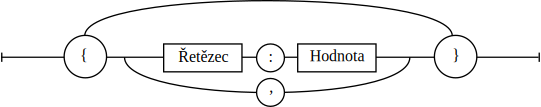
\includegraphics[width=0.8\textwidth]{jsonObject}
\caption{JSON Objekt}
\label{fig:jsonObject}
\end{figure}

\begin{figure}[htb]
\centering
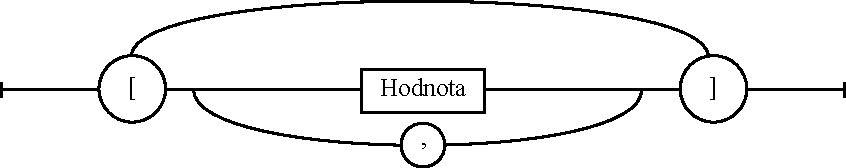
\includegraphics[width=0.8\textwidth]{jsonArray}
\caption{JSON Pole}
\label{fig:jsonArray}
\end{figure}

\begin{figure}[htb]
\centering
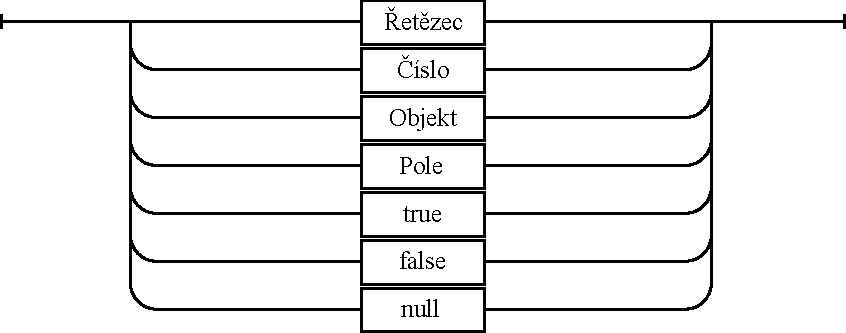
\includegraphics[width=0.8\textwidth]{jsonValue}
\caption{JSON Hodnota}
\label{fig:jsonValue}
\end{figure}

JSON je ve h�e pou�it pro reprezentaci hern�ch �rovn�. Vzhledem k tomu, �e p�i pou�it� jak�hokoliv jin�ho form�tu by bylo pot�eba na vstupu prov�d�t jeho parsov�n�, co� by hru zbyte�n� zpomalovalo, je tento form�t v podstat� jedin�m vhodn�m kandid�tem.

\section{Line�rn� algebra pro 3D grafiku}
\label{section:linearniAlgebra}
Line�rn� algebra je ta ��st matematiky, kter� se zab�v� vektory a maticemi. Pro porozum�n� 3D grafice a WebGL je dobr� m�t alespo� z�kladn� znalosti v tomto oboru. Vzhledem k rozsahu t�to pr�ce nen� mo�n� zm�nit v�e, a proto jsou pojmy jako sou�adn� syst�m, vektory a jejich skal�rn� a vektorov� sou�in pova�ov�ny za znalost �ten��e. N�sleduj�c� text se soust�ed� na homogenn� sou�adnice, matice a transformace ve 3D grafice.

\subsection*{Homogenn� sou�adnice}
\label{subsection:homogenniSouradnice}
V 3D prostoru je mo�n� bod\footnote{Ve 3D grafice naz�van� \textit{vertex}} definovat pomoc� t�� sou�adnic. To v�ak m��e b�t matouc� v tom, �e body a vektory jsou definov�ny stejn�m zp�sobem. S homogenn�mi sou�adnicemi p�id�v�me �tvrtou sou�adnici, kter� je zna�ena jako \textit{w}. Pro vektory je pak $w=0$, a pokud je $w!=0$, pak homogenn� sou�adnice definuj� bod. Homogenn� bod lze p�ev�st na t��prvkov� bod vyd�len�m v�ech sou�adnic sou�adnic� homogenn�. Pro p�evod t��prvkov�ho bodu na bod homogenn� pak sta�� p�idat jako homogenn� sou�adnici hodnotu 1. Homogenn� sou�adnice se pou��vaj� z toho d�vodu, �e ve 3D grafice jsou nej�ast�j�� operac� r�zn� transformace, kter� jsou pops�ny pomoc� $4\times4$ matic. Abychom mohli bod pomoc� t�chto matic transformovat, je nutn�, aby byl bod pops�n pr�v� �ty�mi sou�adnicemi.

\subsection*{Matice}
\label{subsection:matice}
Matice je slo�ena z ��dk� a sloupc�. Elementy uvnit� matice se naz�vaj� prvky matice a dle po�tu ��dk� a sloupc� rozli�ujeme r�zn� jej� dimenze. Nej�ast�ji pou��van�m typem jsou ve WebGL matice se �ty�mi ��dky a �ty�mi sloupci. Tyto pak ozna�ujeme jako $4\times4$ matice.

\begin{equation}
 M = \begin{bmatrix}
       m_{00} & m_{01} & m_{02} & m_{03}     \\[0.3em]
       m_{10} & m_{11} & m_{12} & m_{13}     \\[0.3em]
       m_{20} & m_{21} & m_{22} & m_{23}     \\[0.3em]
       m_{30} & m_{31} & m_{32} & m_{33}     \\[0.3em]
     \end{bmatrix}
\end{equation}

Matic�m s jedn�m sloupcem ($m \times 1$) se tak� jinak ��k� sloupcov� vektor a matic�m s jedn�m ��dkem ��dkov� vektor ($1 \times m$).

\begin{align}
%\begin{split}
 V = \begin{bmatrix}
       v_{0} \\[0.3em]
       v_{1} \\[0.3em]
       v_{2} \\[0.3em]
       v_{3} \\[0.3em]
     \end{bmatrix} \\
%\end{split}
%\begin{split}
V = \begin{bmatrix}
       v_{0} & v_{1} & v_{2} & v_{3}  \\[0.3em]
     \end{bmatrix}
%\end{split}\tag{2.2a, 2.2b} 
\end{align}
%\tag{1a,b} 

\myparagraph{Sou�et a rozd�l matic}
Sou�et a rozd�l je mo�n�, pokud maj� matice stejn� dimenze. Sou�et, nebo rozd�l pak prob�h� prvek po prvku.


\begin{align}
%\begin{split}
 A = \begin{bmatrix}
       1 & 5 & 3 \\[0.3em]
       4 & 4 & 1 \\[0.3em]
     \end{bmatrix} \\
%\end{split}
%\begin{split}
 B = \begin{bmatrix}
       5 & 3 & 3 \\[0.3em]
       2 & 5 & 2 \\[0.3em]
     \end{bmatrix} \\
%\end{split}\tag{2.3a, 2.3b} 
%\end{align}
%\begin{align}
 A + B = \begin{bmatrix}
       6 & 8 & 6 \\[0.3em]
       6 & 9 & 3 \\[0.3em]
     \end{bmatrix}
\end{align}

\myparagraph{N�soben� matic}
N�soben� matic je ve 3D grafice velmi d�le�itou operac�. Definice n�soben� je takov�, �e dv� matice mohou b�t vz�jemn� vyn�sobeny pouze tehdy, kdy� se po�et sloupc� prvn� matice rovn� po�tu ��dk� matice druh�. V�sledn� matice m� pak po�et ��dk� rovn� matici prvn� a po�et sloupc� matici druh�.

\begin{align}
[m \times p][p \times n] = [m \times n]
\end{align}

Prvky \textit{ij} v�sledn� matice vzniknou skal�rn�m vyn�soben�m ��dku \textit{i} matice \textbf{A} a sloupce \textit{j} matice \textbf{B}.

\begin{align}
M = 
\begin{bmatrix*}[r]
  -3 & 1 \\
  -2 & 2 \\
  -4 & 5 \\
\end{bmatrix*} \\
N =
\begin{bmatrix*}[r]
  -4 & 3 \\
   3 & 5 \\
\end{bmatrix*}
\end{align} 
\begin{align}
M \times N = 
\begin{bmatrix*}[r]
  (-3) \times (-4) + 1 \times 3 & (-3) \times 3 + 1 \times 5 \\
  (-2) \times (-4) + 2 \times 3 & (-2) \times 3 + 2 \times 5 \\
  (-4) \times (-4) + 5 \times 3 & (-4) \times 3 + 5 \times 5 \\
\end{bmatrix*}
=
\begin{bmatrix*}[r]
  15 & -4 \\
  14 & 4 \\
  31 & 13 \\
\end{bmatrix*}
\end{align}


\myparagraph{Matice identity a inverzn� matice}
Matice identity je takovou matic�, �e pokud s n� vyn�sob�me jakoukoliv matici jinou, tak z�sk�me op�t tu samou.

\begin{align}
M \times I = I \times M = M
\end{align}

Matice identity je v�dy �tvercov� (stejn� po�et sloupc� jako ��dk�), na sv� diagon�le m� prvky rovny 1 a mimo diagon�lu 0.

\begin{align}
I = 
\begin{bmatrix*}[r]
  1 & 0 & 0 & 0 \\
  0 & 1 & 0 & 0 \\
  0 & 0 & 1 & 0 \\
  0 & 0 & 0 & 1 \\
\end{bmatrix*}
\end{align}

Nyn�, kdy� v�me, co je to matice identity, m��eme p�istoupit k definici matice inverzn�. Pro jak�koliv ��slo $x$ (krom� 0) nalezneme ��slo $1/x$ (zapisov�no tak� jako $x^{-1}$), kter� p�i vyn�soben� touto inverzn� hodnotou d�v� jako sv�j v�sledek hodnotu 1. Podobn� je definov�na i matice inverzn�, kterou ozna�ujeme jako $M^{-1}$.

\begin{align}
M \times M^{-1} = M^{-1} \times M = 1
\end{align}

Je d�le�it� poznamenat, �e pouze �tvercov� matice maj� matici inverzn�.

\myparagraph{Transponovan� matice}
Transponovan� matice vznikne prohozen�m sv�ch ��dk� se sloupci. Matice je definov�na pro jak�koliv dimenze a ozna�uje se jako $M^{T}$. Vzhledem k tomu, �e ve WebGL se pou��vaj� matice $4\times4$, jsou i zde p��klady uvedeny v t�chto dimenz�ch.

\begin{align}
 M = 
\begin{bmatrix*}[r]
  1 & 2 & 3 & 4 \\
  5 & 6 & 7 & 8 \\
  9 & 10 & 11 & 12 \\
  13 & 14 & 15 & 16 \\
\end{bmatrix*}
\end{align}

\begin{align} 
M^T = 
\begin{bmatrix*}[r]
  1 & 5 & 9 & 13 \\
  2 & 6 & 10 & 14 \\
  3 & 7 & 11 & 15 \\
  4 & 8 & 12 & 16 \\
\end{bmatrix*}
\end{align}

\subsection*{Transformace}
\label{subsection:transformace}
Transformace je operace, kter� na sv�m vstupu p�ij�m� jakousi entitu, jakou je nap��klad bod, nebo vektor, a n�jak�m zp�sobem ji modifikuje. Speci�ln�m typem transformace je pak transformace line�rn�, co� je zobrazen� $f$ z jednoho vektorov�ho prostoru do druh�ho $f: V \rightarrow W$, kter� zachov�v� vektorov� operace s��t�n� a n�soben� skal�rem. N�zev \textit{line�rn�} je odvozen z faktu, �e grafem obecn�ho line�rn�ho zobrazen� z re�ln�ch ��sel do re�ln�ch ��sel je p��mka.

M�jme dva vektory $u$, $v$ a transformaci reprezentovanou pomoc� funkce $f$. Pak line�rn� transformac� je operace, kter� spl�uje n�sleduj�c� podm�nky:

\begin{align}
\begin{split}
f(u) + f(v) = f(u+v) 
\end{split}
\begin{split}
 (aditivita)
\end{split} \\
\begin{split}
kf(u) = f(ku)
\end{split}
\begin{split}
 (homogenita)
 \end{split}
\end{align}


Mezi line�rn� transformace pat�� nap��klad posunut� (translace), rotace, zm�na m���tka (scaling), �i zkosen� (shearing). N�soben�m transforma�n�ch matic lze vytv��et ze z�kladn�ch transformac� transformace komplexn�. P�i n�soben� v�ak mus�me d�vat pozor na po�ad�, ve kter�m jsou matice n�sobeny. N�soben� matic toti� nen� komutativn� operac�. Jak�koliv transformace bodu, nebo vektoru v 3D prostoru m��e b�t vyj�d�ena pomoc� $4 \times 4$ matice.

\begin{align} 
Mv = \begin{bmatrix*}[r]
  m_{00} & m_{01} & m_{02} & m_{03} \\
  m_{10} & m_{11} & m_{12} & m_{13} \\
  m_{20} & m_{21} & m_{22} & m_{23} \\
  m_{30} & m_{31} & m_{32} & m_{33} \\
\end{bmatrix*}
\begin{bmatrix*}[r]
 v_{0} \\
 v_{1} \\
 v_{2} \\
 v_{3} \\
\end{bmatrix*} =
\begin{bmatrix*}[r]
  m_{00}v_{0} & m_{01}v_{1} & m_{02}v_{2} & m_{03}v_{3} \\
  m_{10}v_{0} & m_{11}v_{1} & m_{12}v_{2} & m_{13}v_{3} \\
  m_{20}v_{0} & m_{21}v_{1} & m_{22}v_{2} & m_{23}v_{3} \\
  m_{30}v_{0} & m_{31}v_{1} & m_{32}v_{2} & m_{33}v_{3} \\
\end{bmatrix*}
\end{align}

\pagebreak
\myparagraph{Translace}
Translace je line�rn� transformac�, kter� posouv� bod v prostoru. Transla�n� matice vypad� n�sledovn�:

\begin{align}
T(t_x, t_y, t_z) = 
\begin{bmatrix*}[r]
 1 & 0 & 0 & t_x \\
 0 & 1 & 0 & t_y \\
 0 & 0 & 1 & t_z \\
 0 & 0 & 0 & 1 \\
\end{bmatrix*}
\end{align}

Uveden� transla�n� matice posouv� bod s ofsetem, kter� je reprezentov�n pomoc� vektoru $(t_x, t_y, t_z)$. Diagram~\ref{fig:translation} zn�zor�uje translaci bod� krychle n�soben�m s n�sleduj�c� matic�:

\begin{align}
T(4, 5, 0) = 
\begin{bmatrix*}
1 & 0 & 0 & 5 \\
0 & 1 & 0 & 0 \\
0 & 0 & 1 & 0 \\
0 & 0 & 0 & 1 \\
\end{bmatrix*}
\end{align}

\begin{figure}[htb]
\centering
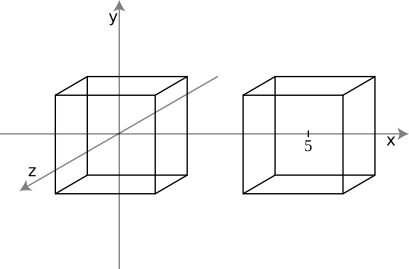
\includegraphics[width=0.8\textwidth]{translation}
\caption{Translace}
\label{fig:translation}
\end{figure}


\subsection*{Rotace}
Tato transformace rotuje bod, �i vektor o zadan� �hel kolem po��tku sou�adn�ho syst�mu $[0, 0, 0]$. B�n� se pou��vaj� rota�n� matice pro rotaci kolem osy\footnote{Rotace se ��d� tzv. pravidlem prav� ruky. Palec sm��uje v kladn�m sm�ru osy a zbyl� zato�en� prsty ruky nazna�uj� sm�r kladn� rotace.} x, y a z. 

\begin{align}
R_x(\phi) = 
\begin{bmatrix*}
1 & 0 & 0 & 0 \\
0 & \cos\phi & -\sin\phi & 0 \\
0 & \sin\phi & \cos\phi & 0 \\
0 & 0 & 0 & 1 \\
\end{bmatrix*}
\end{align}

\begin{align}
R_y(\phi) = 
\begin{bmatrix*}
\cos\phi & 0 & \sin\phi & 0 \\
0 & 1 & 0 & 0 \\
-\sin\phi & 0 & \cos\phi & 0 \\
0 & 0 & 0 & 1 \\
\end{bmatrix*}
\end{align}

\begin{align}
R_z(\phi) = 
\begin{bmatrix*}
\cos\phi & -\sin\phi & 0 & 0 \\
\sin\phi & \cos\phi & 0 & 0 \\
0 & 0 & 1 & 0 \\
0 & 0 & 0 & 1 \\
\end{bmatrix*}
\end{align}

Diagram~\ref{fig:rotation} zn�zor�uje rotaci bod� krychle kolem po��tku soustavy sou�adnic s vyu�it�m t�to transforma�n� matice:

\begin{align}
R_x(30^{\circ}) = 
\begin{bmatrix*}
1 & 0 & 0 & 0 \\
0 & \cos(30^{\circ}) & -\sin(30^{\circ}) & 0 \\
0 & \sin(30^{\circ}) & \cos(30^{\circ}) & 0 \\
0 & 0 & 0 & 1 \\
\end{bmatrix*}
\end{align}

\begin{figure}[htb]
\centering
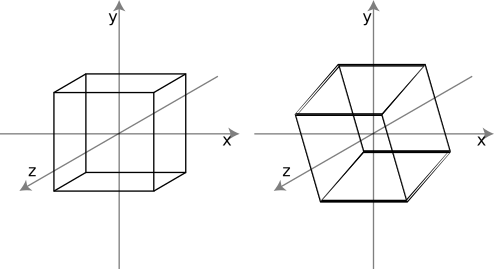
\includegraphics[width=0.8\textwidth]{rotation}
\caption{Rotace}
\label{fig:rotation}
\end{figure}

Dal��mi transformacemi pou��van�mi ve 3D grafice je tzv. scaling, kter� zv�t�uje, �i zmen�uje objekt a pak tzv. shearing, kter� dok�e objekt zkosit dle dan� osy. Tyto dv� transformace v�ak nejsou p�i implementaci hry vyu�ity, a tud�� zde nebudou zm�n�ny.

\pagebreak
\section{WebGL}
\label{section:webgl}
WebGL je n�zko�rov�ov� aplika�n� rozhran� pro zobrazen� pokro�il� 3D grafiky na webu. Je zalo�eno na OpenGL ES 2.0 a umo��uje program�torovi pou��t hardwarov� akcelerovan�\footnote{K hardwarov� akceleraci je nutno vlastnit GPU s podporou minim�ln� shader modelu 2.0. V opa�n�m p��pad� lze obraz vykreslovat softwarov�.} vykreslov�n� obrazu v kontextu HTML a JavaScriptu. Vykreslovac� plochou, kter� je zde pou�ita je HTML5 \texttt{<canvas>} element a jeho \texttt{webgl}, resp. \texttt{experimental-webgl} kontext.~\cite{seidelin2011html5}

\subsection*{Historie WebGL}
\label{subsection:historieWebGL}
Prvn� experimenty s 3D grafikou v \texttt{<canvas>} elementu prov�d�l Vladimir Vuki�evi� ze spole�nosti Mozilla. V�sledkem jeho pokus� se stal prototyp, kter� nazval Canvas 3D. V roce 2009 vytvo�ila Khronos Group novou pracovn� skupinu pro WebGL, kter� byla slo�ena z hlavn�ch tv�rc� webov�ch prohl��e�� v�etn� firem jako Apple, Google, Mozilla a Opera. Khronos Group je neziskovou organizac�, kter� vytv��� a spravuje otev�en� standardy a aplika�n� rozhran�. Byla zalo�ena roku 2000 a mimo jin� stoj� i za standardy jako OpenGL, �i v��e zm�n�n�m OpenGL ES, kter� je prim�rn� ur�eno pro vestav�n� syst�my.~\cite{anyuru2012professional}

Fin�ln� specifikace WebGL 1.0\footnote{\url{http://www.khronos.org/registry/webgl/specs/1.0/}} byla vyd�na v b�eznu roku 2011 a jej� implementaci m��eme nal�zt v prohl��e��ch jako Google Chrome, Mozilla Firefox, Safari a v po��te�n�ch f�z�ch implementace v prohl��e�i Opera. V p��pad� Microsoft Internet Exploreru je situace pon�kud odli�n�. Microsoft neohl�sil ��dn� z�m�r v podpo�e WebGL ve sv�m prohl��e�i. U�ivatel�, kte�� cht�j� WebGL pou��vat, jsou tedy nuceni p�ej�t k jin�mu prohl��e�i.~\cite{anyuru2012professional}

\subsection*{V�hody WebGL}
\label{subsection:vyhodyWebGL}
V dob�ch, kdy web jako takov� za��nal, byl jeho obsah vytvo�en ze statick�ch dokument�. Hlavn� prac� webov�ch prohl��e�� tehdy bylo takov�to obsah z�skat a zobrazit. V pr�b�hu �asu v�ak webov� technologie zna�n� pokro�ily a nyn� tak jejich prost�ednictv�m m��eme p�istupovat k plnohodnotn�m webov�m aplikac�m s bohat�m u�ivatelsk�m rozhran�m a audiovizu�ln�m obsahem. Tyto aplikace se nyn� st�vaj� alternativou k aplikac�m nativn�m.~\cite{anyuru2012professional} \\ \\
Jejich hlavn�mi v�hodami jsou:
\begin{itemize}
\item Rychl� \textbf{dostupnost} a jednoduch� \textbf{distribuce} mezi mnoho u�ivatel�.
\item \textbf{Snadn� �dr�ba a aktualizace aplikac�.} Pokud je v aplikaci nalezena chyba, nebo pokud chceme roz���it jej� funkcionalitu, pak v�e, co je pot�eba, je aktualizovat aplikaci na serveru a u�ivatel� maj� ihned p��stup k jej� nov� verzi.
\item \textbf{Multiplatformnost aplikac�.} V�e, co u�ivatel pot�ebuje je kompatibiln� webov� prohl��e� schopn� zobrazit n�mi definovan� obsah.
\end{itemize}

Oproti nativn�m aplikac�m nejsou ty webov� obsahem tak bohat�, av�ak s p��chodem HTML5 za��n� tento rozd�l mizet. Prost�ednictv�m WebGL je nyn� mo�n� zobrazovat hardwarov� akcelerovanou grafiku p��mo uvnit� prohl��e�e. Je tak mo�n� vytvo�it 3D hry, nebo pokro�il� 3D grafick� aplikace a z�rove� t�it z v�hod webu, jak byli pops�ny v��e. Technologie WebGL m� nav�c i dal�� v�hody, mezi n� pat�� nap��klad:
\begin{itemize}
\item WebGL je otev�en� standard, kter� m��e pou��vat ka�d� bez poplatk�.
\item WebGL vyu��v� p��mo grafick� hardware, co� znamen�, �e jsou aplikace rychl�.
\item Vzhledem k tomu, �e je WebGL zalo�eno na OpenGL ES, je mo�n� vytvo�en� aplikace spou�t�t i na mnoh�ch modern�ch mobiln�ch za��zen�ch.
\end{itemize}

\subsubsection*{Grafick� API}
\label{subsection:grafickaAPI}
Existuj� dva fundament�ln� p��stupy, kter� jsou u grafick�ch aplika�n�ch rozhran� vyu�ity. Jsou jimi:
\begin{itemize}
\item immediate-mode API a 
\item retained-mode API,
\end{itemize}
p�i�em� WebGL pou��v� prvn� ze zm�n�n�ch p��stup�.


\myparagraph{Immediate-mode API} 
U tohoto typu rozhran� je cel� sc�na p�ekreslena s ka�d�m sn�mkem bez ohledu na to, zda byla zm�n�na, �i nikoliv. Grafick� knihovna kter� zprost�edkov�v� rozhran� program�torovi neukl�d� ��dnou intern� reprezentaci sc�ny, kter� m� b�t vykreslena. Reprezentaci sc�ny je tak nutn� uchov�vat v pam�ti vlastn� aplikace. Tento p��stup je vysoce flexibiln� a poskytuje program�torovi v�t�� �rove� kontroly nad v�sledn�m vykreslovan�m obrazem. Na druhou stranu v�ak tento p��stup vy�aduje ze strany program�tora v�ce �sil� oproti p��stupu, kter� si pop��eme nyn�.

\begin{figure}[htb]
\centering
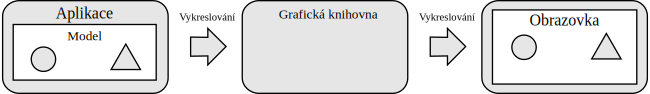
\includegraphics[width=0.8\textwidth]{immediateMode}
\caption{Immediate-mode API}
\label{fig:immediateMode}
\end{figure}

\myparagraph{Retained-mode API} 
U tohoto p��stupu je intern� model a ve�ker� vykreslovan� objekty sc�ny obsa�en v grafick� knihovn�, kter� toto rozhran� program�torovi nab�z�. Program�tor vyu��v� p��stupov�ch metod k rozhran� a knihovna sama rozhoduje o tom, zda m� b�t sc�na a s n� jej� intern� reprezentace aktualizov�na, �i nikoliv. To znamen�, �e aplikace, kter� rozhran� vyu��v�, nemus� v ka�d�m vykreslovan�m sn�mku sc�nu p�ekreslovat. Tento p��stup je v mnoh�ch ohledech pro program�tora m�n� n�ro�n� a pou��v� se nap��klad pro vykreslov�n� vektorov� grafiky (SVG). 

\begin{figure}[htb]
\centering
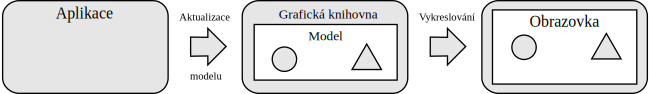
\includegraphics[width=0.8\textwidth]{retainedMode}
\caption{Retained-mode API}
\label{fig:retainedMode}
\end{figure}
 
\subsection*{Tvorba obrazu v grafick�m hardwaru}
\label{subsection:tvorbaObrazu}
WebGL je n�zko�rov�ov� rozhran� a pracuje tak velmi bl�zko grafick�ho hardwaru. K pochopen� fundament�ln�ch koncept� pou�it�ch p�i implementaci hry je tedy nejprve pot�eba alespo� okrajov� osv�tlit, jak�m zp�sobem grafick� hardware pracuje. 

Na diagramu~\ref{fig:gpuDisplay} je zjednodu�en� zn�zorn�n vztah grafick�ho hardwaru k ostatn�m ��stem syst�mu.

\begin{figure}[htb]
\centering
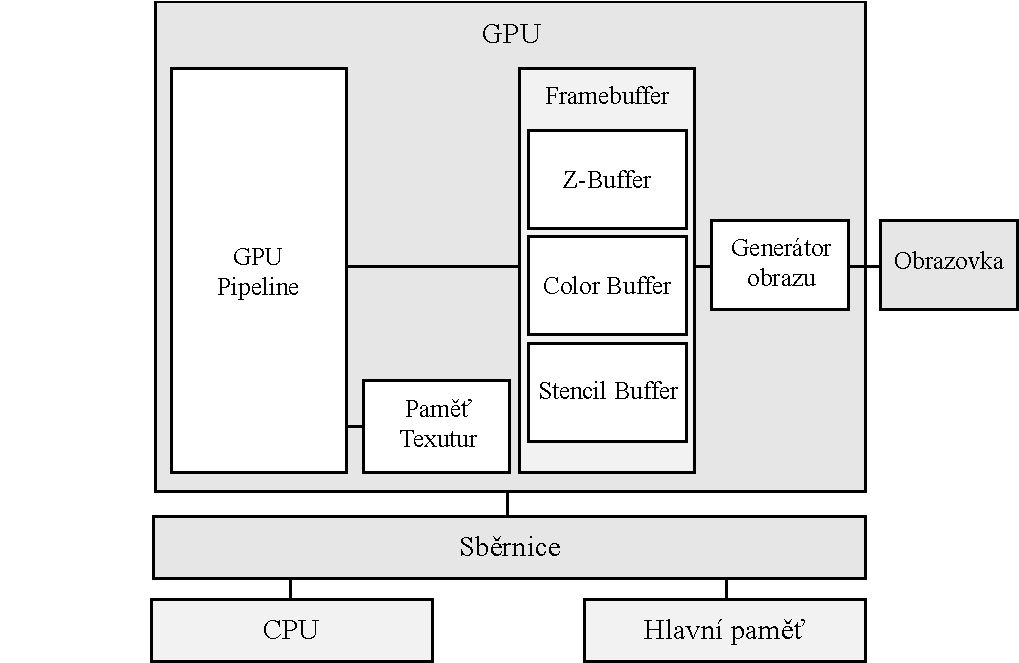
\includegraphics[width=0.8\textwidth]{gpuDisplay}
\caption{Vztah grafick�ho hardwaru k ostatn�m ��stem syst�mu}
\label{fig:gpuDisplay}
\end{figure}

\myparagraph{GPU}
GPU, neboli tak� Graphics Processing Unit, je dedikovan� za��zen�, kter� je p��mo navr�eno pro zobrazen� grafiky. Architektura GPU je vysoce paralelizovan� a prov�d� operace s grafick�mi daty velmi rychle. Zpracov�n� dat prob�h� typicky z�et�zen� v n�kolika �rovn�ch.

\myparagraph{Framebuffer}
Framebuffer je m�stem, kde je ulo�en v�sledek operac� proveden�ch na GPU. Je to pam�, kter� obsahuje informace nutn� pro zobrazen� v�sledn�ho obrazu na zobrazovac� za��zen�. V jednoduch�m grafick�m syst�mu m��e b�t fyzick� pam� framebufferu sou��st� hlavn� opera�n� pam�ti, av�ak u modern�ch syst�m� je tato pam� alokov�na ve speci�ln� rychl� grafick� pam�ti na GPU. Framebuffer se typicky skl�d� ze t�� odli�n�ch \textit{subbuffer�}.

\begin{itemize}
\item Color Buffer
\item Z-Buffer
\item Stencil Buffer
\end{itemize}

\mysubparagraph{Color Buffer}
Color buffer p�edstavuje dvourozm�rn� pole, jeho� prvky jsou v�sledn� barvy pixel� obrazu. Ka�d� z t�chto prvk� obsahuje informaci o v�sledn� barv� v RGB, �i RGBA form�tu. Ka�d� z barevn�ch kan�l� m� alokov�n ur�it� po�et bit� a nav�c m��e b�t obsa�ena informace o \textit{alpha} kan�lu, kter� ur�uje viditelnost dan�ho pixelu. Celkov� po�et bit� pou�it�ch pro jeden pixel je ozna�ov�n jako barevn� hloubka (color depth). \\ \\ Varianty barevn� hloubky:

\begin{itemize}
\item 16 bit� na pixel
\item 24 bit� na pixel
\item 32 bit� na pixel
\end{itemize} 

Barevn� hloubka 16 bit� se �asto pou��v� na men��ch za��zen�ch. Je zde pou�ito syst�mu RGB565, kter� zohled�uje zv��enou citlivost lidsk�ho oka na zelenou barvu. Rozlo�en� jednotliv�ch barevn�ch kan�l� tedy nen� rovnom�rn� a je alokov�no 5 bit� pro �ervenou barvu, 6 bit� pro barvu zelenou a 5 bit� pro barvu modrou. Barevn� hloubka 24 bit� m� pak pro ka�dou barvu alokov�no po osmi bitech a v p��pad� barevn� hloubky 32 bit� je dal��ch 8 bit� alokov�no pro alpha kan�l.

\mysubparagraph{Z-Buffer}
Jak ji� bylo uvedeno v p�edchoz�m odstavci, color buffer typicky obsahuje barvy pixel� v�sledn�ho obrazu. V zobrazovan� sc�n� jsou v�ak n�kter� vykreslovan� objekty p�ekryty jin�mi a pixely, kter� t�mto zakryt�m objekt�m n�le��, by tak nem�ly b�t viditeln�. Toho je doc�leno pomoc� z-bufferu, kter� m� stejn� po�et prvk� jako color buffer, av�ak nen� zde ulo�ena barva, n�br� vzd�lenost pozorovatele od nejbli���ho objektu sc�ny. Ta n�sledn� rozhoduje o tom, jak� objekt m� b�t v dan�m pixelu vykreslen a kter� nikoliv. V souvislosti s implementac� je tento buffer vyu��v�n pouze v p��pad�, �e objekty sc�ny nejsou zpr�hledn�ny.

\mysubparagraph{Stencil Buffer}
Jako dopln�k ke d��ve popsan�m buffer�m je na modern�m grafick�m hardwaru p��tomen i stencil buffer, kter� ur�uje to, kam m� b�t aktu�ln� zpracov�van� objekt sc�ny vykreslen v r�mci color bufferu. V praxi je tento buffer vyu�it nap��klad pro vykreslov�n� st�n�. St�ny nejsou v implementaci pou�ity, proto se ji� d�le stencil bufferem nebudeme zab�vat.

\subsection*{Grafick� pipeline}
\label{subsection:pipeline}
Webov� aplikace jsou typicky slo�eny z HTML, CSS a JavaScriptov�ch soubor�, kter� jsou interpretov�ny a zobrazov�ny prohl��e�em. Aplikace vyu��vaj�c� WebGL nav�c obsahuje zdrojov� k�d shader� a data, kter� reprezentuj� 3D sc�nu. JavaScript vyu��v� rozhran� WebGL, aby p�edal t�to knihovn� zdrojov� k�dy programovateln�ch sou��st� grafick� pipeline a data, kter� reprezentuj� vykreslovan� 3D model. Pot�, co jsou data knihovn� p�ed�na, je v�sledek vykreslen do tzv. \textit{drawing bufferu}, co� je ve sv� podstat� framebuffer pro WebGL. Stejn� tak jako framebuffer obsahuje color, stencil a z-buffer, av�ak jeho obsah je nejd��ve spojen se zbytkem webov� str�nky a teprve pot� kon�� ve framebufferu fyzick�m. V implementaci hry je vyu�ito 32 bitov� varianty drawing bufferu a je tak tedy mo�n� vyu��t alpha kan�lu na prol�n�n� vykreslovan� 3D grafiky se sv�m okol�m, resp. se zbytkem webov� str�nky. Grafick� pipeline je zobrazena na diagramu~\ref{fig:gpuPipeline}.

\begin{figure}[htb]
\centering
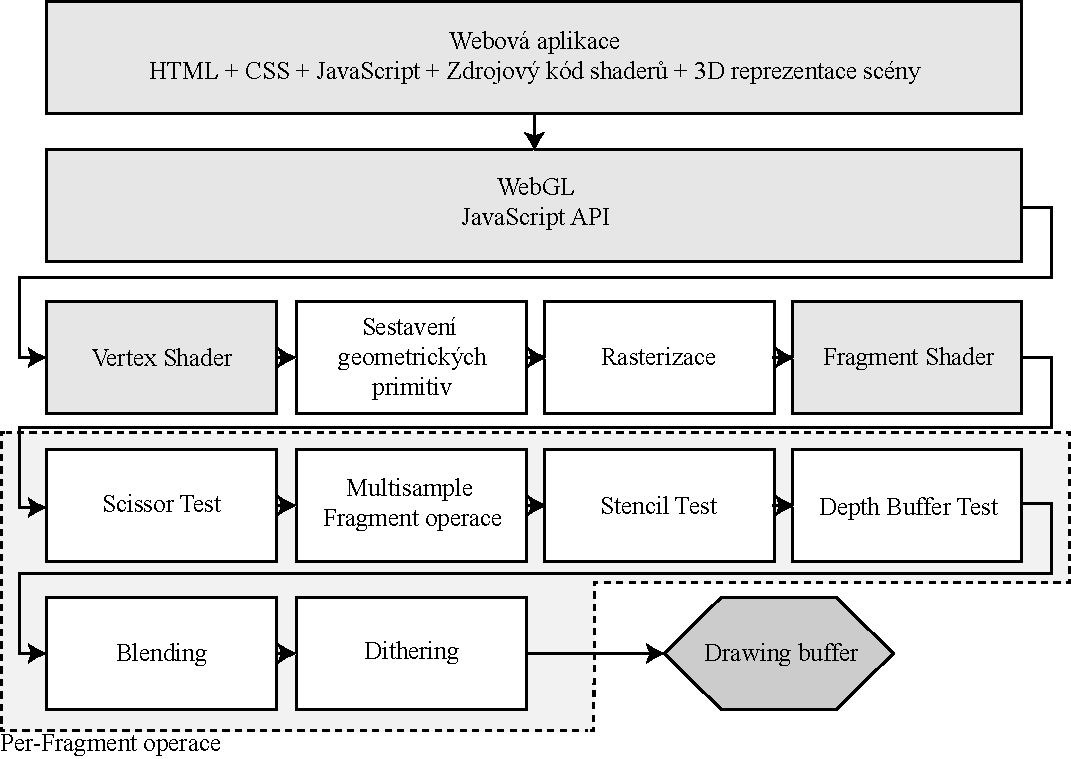
\includegraphics[width=0.8\textwidth]{gpuPipeline}
\caption{GPU pipeline}
\label{fig:gpuPipeline}
\end{figure}

K tomu, abychom z�skali realistickou 3D sc�nu nesta�� pouze vykreslit objekty na ur�it� pozice. Mus�me tak� vz�t v �vahu, jak budou objekty vypadat, pokud na n� bude dopadat sv�tlo ze sv�teln�ch zdroj� sc�ny. Obecn� se technice, kter� se pou��v� ve spojitosti s p�soben�m sv�tla na r�zn� typy materi�l� ��k�~\textit{shading}. Ve WebGL je shading rozd�len do dvou ��st�, jejich� chov�n� je mo�n� naprogramovat. \\ \\ Programovateln�mi sou��stmi grafick� pipeline jsou:
\begin{itemize}
\item Vertex Shader
\item Fragment Shader
\end{itemize}

\myparagraph{Vertex Shader}
Prvn� ��st� grafick� pipeline, do kter� vstupuj� data p�edan� WebGL knihovn�, je vertex shader. Jak ji� jeho n�zev napov�d�, prov�d� shading jednotliv�ch vertex� vykreslovan� sc�ny. Ne� v�ak samotn� proces shadingu zapo�ne, je nutno vertexy transformovat a um�stit tak objekt, jemu� vertexy n�le��, na po�adovanou pozici. Toho je doc�leno pomoc� transforma�n�ch matic, kter� jsou pops�ny v podkapitole~\ref{section:linearniAlgebra}. Vertex shader pou��v� n�sleduj�c� vstupy:
\begin{itemize}
\item Zdrojov� k�d vertex shaderu, kter� je zaps�n v OpenGL ES Shading Language (GLSL ES).
\item Atributy, kter� definuj� data specifick� ka�d�mu vertexu. Typicky je to jeho pozice, norm�la a barva.
\item Tzv. \textit{uniform} prom�nn�, kter� jsou pro v�echny vertexy objektu konstantn� a lze je zm�nit a� po dokon�en� operace vykreslov�n�. Jedn� se o transforma�n� matice a d�le pak nap��klad o pozice, na kter�ch se nach�z� sv�teln� zdroje.
\end{itemize}

\begin{figure}[htb]
\centering
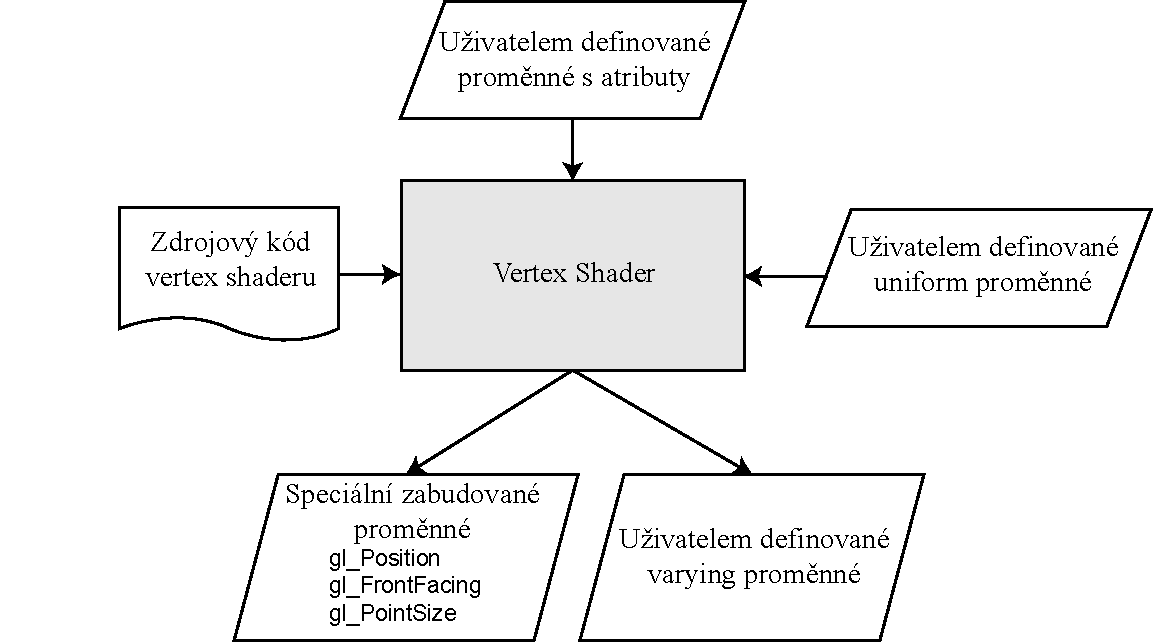
\includegraphics[width=0.8\textwidth]{vertexShader}
\caption{Vertex Shader}
\label{fig:vertexShader}
\end{figure}

Na diagramu~\ref{fig:vertexShader} jsou pak jest� zn�zorn�ny zabudovan� a u�ivatelky definovan� \textit{varying} prom�nn�. Vyu�it� varying prom�nn�ch je v delegaci informac� z vertex shaderu do fragment shaderu. Jednou z nejd�le�it�j��ch speci�ln�ch zabudovan�ch prom�nn�ch je \texttt{gl\_Position}, kter� po pr�ci vertex shaderu ud�v� pozici, na kter� se vertex nach�z�. Popis vertex shaderu prob�h� pomoc� jazyka GLSL, kter� je svou syntax� podobn� programovac�mu jazyku C. P��klad takov�ho popisu je uveden ve zdrojov�m k�du~\ref{code:vertexShader}

\begin{lstlisting}[caption=Uk�zka zdrojov�ho k�du GLSL pro vertex shader,label=code:vertexShader]
// Deklarace atribut� vertexu
// Vektor pozice vertexu (XYZ)
attribute vec3 aVertexPos;
// Barva vertexu (RGBA)
attribute vec4 aVertexColor;

// Uniform prom�nn�
// Model-View Matice (4x4)
uniform mat4 uMVMatrix;
// Projek�n� matice (4x4)
uniform mat4 uPMatrix;

// Deklarace varying prom�nn� obsahuj�c� v�stupn� barvu vertexu, 
// kter� je vstupem pro fragment shader.
varying vec4 vColor;

void main() {
	// Transformace vertexu projek�n� a model-view matic�, kde
	// gl_Position ud�v� jeho v�slednou pozici ve sc�n�.
	gl_Position = UPMatrix * uMVMatrix * vec4(aVertexPos, 1.0);
	
	// Barva vertexu je posl�na d�le do fragment shaderu	.
	vColor = aVertexColor;
}
\end{lstlisting}
\pagebreak
\myparagraph{Sestaven� primitiv}
V tomto kroku jsou sestaveny jednotliv� vertexy, kter� pro�ly skrze vertex shader, do geometrick�ch primitiv, jak�mi jsou nap��klad troj�heln�ky �i hrany. N�sledn� je pot�eba rozhodnout o tom, zda je sestaven� objekt v regionu, kter� je aktu�ln� viditeln� na obrazovce. Tento region je ozna�ov�n jako \textit{frustrum} a je p�edstavov�n komol�m jehlanem s obd�ln�kovou, �i �tvercovou podstavou. Objekt kter� je uvnit� frustra je p�ed�n ke zpracov�n� dal��m ��stem grafick� pipeline. Objekty, kter� jsou kompletn� mimo frustrum, se odstran�, a ty, kter� jsou vn� pouze ��ste�n�, budou o��znuty. Frustrum je zn�zorn�no na diagramu~\ref{fig:frustrum}

\begin{figure}[htb]
\centering
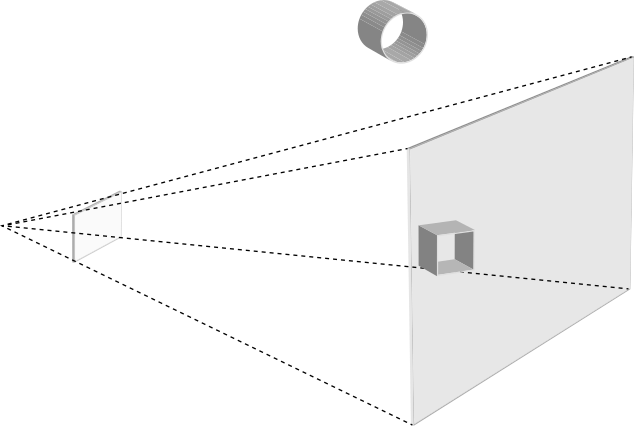
\includegraphics[width=0.8\textwidth]{frustrum}
\caption{Frustrum}
\label{fig:frustrum}
\end{figure}

\myparagraph{Rasterizace}
Dal��m krokem je p�evod primitiv na fragmenty (diagram~\ref{fig:planeFragment}), pod kter�mi si m��eme p�edstavit jednotliv� pixely obrazovky. Fragmenty d�le putuj� do fragment shaderu.

\begin{figure}[htb]
\centering
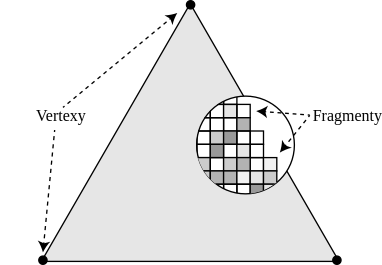
\includegraphics[width=0.8\textwidth]{planeFragment}
\caption{Fragmenty}
\label{fig:planeFragment}
\end{figure}

\myparagraph{Fragment shader}
Fragment shader je druhou programovatelnou sou��st� grafick� pipeline. Jak ji� bylo zm�n�no, fragment odpov�d� pixelu, av�ak ne v�echny fragmenty se pixely stanou. Fragmenty toti� mohou b�t odstran�ny v dal��ch ��stech pipeline. Fragment shader se sv�mi vstupy a v�stupy je zn�zorn�n na diagramu~\ref{fig:fragmentShader}. Vstupem fragment shaderu jsou:
\begin{itemize}
\item Zdrojov� k�d fragment shaderu v jazyku OpenGL ES Shading Language.
\item Speci�ln� zabudovan� prom�nn�, mezi n� pat�� nap��klad \texttt{gl\_PointCoord}.
\item Varying prom�nn�, kter� byli posl�ny skrze vertex shader.
\item Uniform prom�nn�, kter� obsahuj� konstanty spole�n� v�em fragment�m vykreslovan�ho objektu.
\item Samplery, co� jsou speci�ln� uniform prom�nn� ur�en� pro texturov�n�.
\end{itemize}

\begin{figure}[htb]
\centering
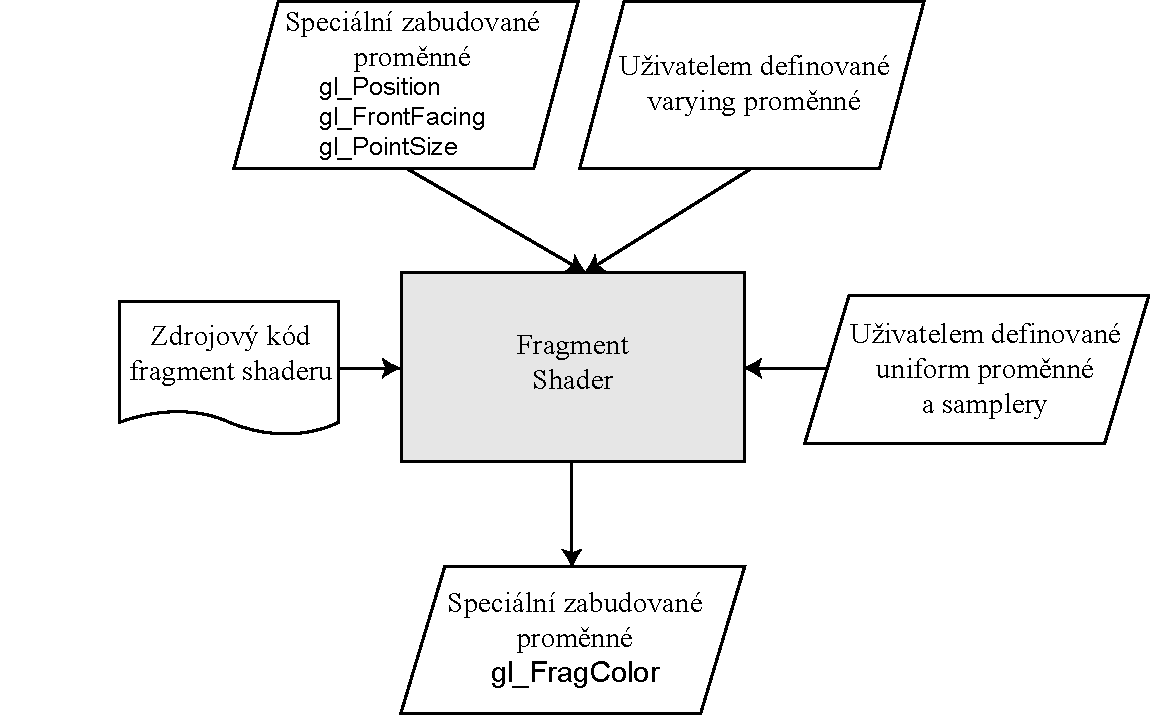
\includegraphics[width=0.8\textwidth]{fragmentShader}
\caption{Fragment Shader}
\label{fig:fragmentShader}
\end{figure}



Jak ji� bylo zm�n�no d��ve, varying prom�nn� slou�� k pos�l�n� informac� skrze vertex shader. Obecn� v�ak plat�, �e objekt m� v�ce fragment� ne� vertex�. Obsah varying prom�nn�ch, kter� je zasl�n skrze vertex shader, je line�rn� interpolov�n pro ka�d� fragment. 

V�sledek pr�ce fragment shaderu je zaps�n do zabudovan� prom�nn� \texttt{gl\_FragColor}, kter� n�sledn� obsahuje v�slednou barvu dan�ho fragmentu. Ve zdrojov�m k�du~\ref{code:fragmentShader} je uveden p��klad GLSL programu fragment shaderu, kter� pro ka�d� fragment z�sk� line�rn� interpolovanou hodnotu s jeho barvou a ulo�� ji jako sv�j v�stup.

\label{code:fragmentShader}
\begin{lstlisting}[caption=P��klad jednoduch�ho GLSL programu fragment shaderu]
varying ver4 vColor;
void main(){
	gl_FragColor = vColor;
}
\end{lstlisting}

\myparagraph{Per-Fragment operace}
Ka�d� fragment, kter� projde fragment shaderem, je postoupen do dal��ho bloku pipeline, kter� se skl�d� z n�kolika ��st� prov�d�j�c� tzv. per-fragment operace. Ka�d� z operac� m��e ovlivnit v�sledn� pixel v drawing bufferu, av�ak v implementaci je vyu�ito pouze blendingu a depth buffer testu. Zbyl� ��sti jsou uvedeny pro �plnost popisu pipeline.

\mysubparagraph{Scissor test}
Scissor test ur�uje, zda je zpracov�van� fragment uvnit� pravo�hl�ho rovnob�n�ku, kter� je definov�n jedn�m bodem, v��kou a ��rkou. Fragmenty mimo tento rovnob�n�k jsou zahozeny, ostatn� pokra�uj� d�le v cest� grafickou pipeline.

\mysubparagraph{Multisample fragment operace}
Tato ��st pipeline modifikuje aplha kan�l fragmentu, ��m� je doc�leno vyhlazen� hran vykreslovan�ch objekt�. Tato technika se obecn� ozna�uje jako \textit{anti-aliasing}.

\mysubparagraph{Stencil test}
Zde se fragment porovn�v� s nastavenou referen�n� hodnotou. Na z�klad� v�sledku porovn�n� je fragment op�t zahozen, nebo postoupen d�le.

\mysubparagraph{Depth buffer test}
Vzhledem k tomu, �e se v t�m�� ka�d� vykreslovan� sc�n� objekty p�ekr�vaj�, je nutn� do color bufferu vykreslovat pouze ty objekty, kter� jsou viditeln�. Tento test ve spolupr�ci s depth bufferem rozhoduje o tom, zda fragment vykreslovat, �i nikoliv.

\mysubparagraph{Blending}
V dal��m kroku ozna�ovan�m jako blending jsou kombinov�ny barvy fragment�, kter� jsou moment�ln� vykresleny do color bufferu na odpov�daj�c� pozici. Toho je v implementaci vyu�ito pro vykreslov�n� pr�hledn�ch objekt� sc�ny.

\mysubparagraph{Dithering}
Posledn�m krokem p�ed vykreslen�m do color drawing bufferu je tzv. dithering. Vzhledem k tomu, �e color buffer m� omezen� po�et bit� k reprezentaci ka�d� z barev, dithering tyto slo�� tak, �e vytvo�� iluzi toho, �e m�me k dispozici barev v�ce.

%\subsection*{WebGL Frameworky}
%\label{subsection:webGLFrameworky}
%Specifikace neexistuje dlouhou dobu, av�ak ji� dnes m��eme nal�zt mnoh� frameworky, kter� programov�n� s WebGL zna�n� usnad�uj�. Vzhledem k tomu, �e pou�it� WebGL framework� nebylo p�i implementaci povoleno, m� n�sleduj�c� p�ehled pouze informativn� charakter.

%Mezi nejzn�m�j�� WebGL frameworky pat��:
%\begin{itemize}
%\item C3DL
%\item Copperlicht
%\item GLGE
%\item SceneJS
%\item Three.js
%\item WebGLU
%\end{itemize}

%\subsection*{WebGL a bezpe�nost}
%WebGL p�istupuje p��mo ke grafick�mu hardwaru, tud�� se mohou objevit situace, ve kter�ch je mo�n� tuto skute�nost zneu��t a vytvo�it takov� %WebGL dokument, kter� zp�sob� to, �e grafick� karta p�estane reagovat na ostatn� aplikace. Syst�my Microsoft Windows tuto skute�nost detekuj� a %resetuj� grafickou kartu, av�ak na syst�mech firmy Apple nen� tato detekce p��tomna a takov� dokument by potenci�ln� mohl zap���init p�d %syst�mu. U Linuxu z�le�� na verzi pou�it�ho ovlada�e grafick� karty. N�kter� z nich blokaci detekuj� a n�kter� nikoliv (nap��klad sou�asn� %ovlada� grafick�ch karet NVIDIA Nouveau). 

%\subsection*{Rychlost JavaScriptu v souvislosti s WebGL}
%Interprety JavaScriptu v prohl��e��ch se neust�le vylep�uj� a dosahuj� tak vy���ch rychlost�, av�ak pro v�po�etn� slo�it� operace je jeho %rychlost st�le n�zk�. Pokud tedy chceme dos�hnout rychl�ho vykreslov�n�, je pot�eba p�enechat co nejv�ce pr�ce grafick�mu hardwaru a jeho %shader�m. Na diagramu~\ref{webglPerformace} je uvedeno srovn�n� jednotliv�ch webov�ch prohl��e�� s  

%doplnit osvetlovaci modely a opacity



\chapter{Koncepce hry}
\label{chap:analysis}
Návrh implementované hry zakládá na analýze hry Berušky 2, která byla provedena metodou \textit{černé skříňky}\footnote{Na základě akcí uživatele byla zkoumána reakce hry s tím, že princip vnitřní implementace zůstal utajen.}. Hra je nejprve stručně představena a následně jsou uvedeny výsledky herní analýzy, na kterých zakládá implementace~\ref{chap:implementace}

\section{Berušky 2}
Berušky 2, neboli také Berušky 3D, jsou pokračováním logické hry vývojářského týmu Anakreon\footnote{\url{www.anakreon.cz}}, jehož členem je pan Ing. Martin Stránský, který byl konzultantem této bakalářské práce. Oproti své první, volně dostupné verzi, bylo toto pokračování od počátku vytvářeno jako komerční produkt. Hra byla od roku 2004 distribuována v České republice a některých dalších zemích společností Cinemax. V březnu roku 2011 byla část této hry uvolněna pod open-source licencí a je dále vyvíjena panem Stránským. První verze hry Berušky je svou koncepcí velmi podobná hře Sokoban~\footnote{\url{https://en.wikipedia.org/wiki/Sokoban}}. Druhá verze hry se svou koncepcí příliš od prvního dílu neodlišuje, avšak do hry přibyly nové herní prvky, a co je hlavní, hra je kompletně ve 3D. Každá úroveň této hry je logickou hříčkou, která ke svému řešení vyžaduje volbu správného plánu a dávku trpělivosti. Každá z berušek má schopnost před sebou tlačit bedny a používat herní předměty, čímž vytváří cestu k cíli, avšak pro jeho dosažení je často důležité, aby spolu berušky vzájemně spolupracovali.

Původní hra distribuovaná firmou Cinemax obsahuje celkově 160 herních úrovní včetně 20 tutoriálů a 45 jednodušších úrovní, které jsou určeny pro mladší hráče a trénink. Hlavní součástí hry je pak \textit{Beruščí cesta}, která obsahuje celkem 95 úrovní rozdělených do 9 epizod odehrávajících se v různých prostředích. Open-source verze hry pak obsahuje tutoriály, některé tréninkové úrovně a 3 z úrovní Beruščí cesty.

\section{Herní pole}
Herní pole je ve tvaru krychle či kvádru a je rozděleno na jednotlivé pozice, ve kterých jsou umístěny jeho prvky (diagram~\ref{fig:gameField}). Nikdy nemůže dojít k situaci, že by se herní prvek včetně berušek vyskytl mimo herní pole. Po prvcích jako jsou bedny, či zeď je možné se volně pohybovat, avšak beruška nikdy nemůže z vyšší herní pozice seskočit dolů.

\begin{figure}[htb]
\centering
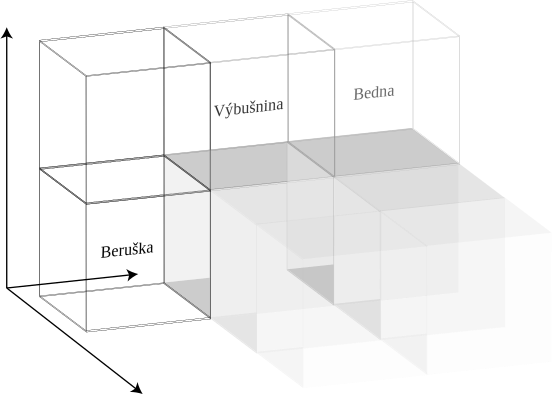
\includegraphics[width=0.8\textwidth]{gameField}
\caption{Herní pole a jeho prvky}
\label{fig:gameField}
\end{figure}

\section{Prvky herního pole}
Jak již bylo uvedeno, v rámci herního pole jsou umístěny prvky, jejichž rozmístění představuje samotnou logickou hříčku, kterou hráč řeší. Prvky se od sebe liší nejen funkčností a vzhledem, ale také tím, že některé z nich jsou umístěny staticky (hráč s nimi nemůže pohnout) a některé z nich jsou dynamické (bedny, výbušniny, \ldots). Následuje přehled prvků herního pole a jejich stručný popis.

\myparagraph{Beruška}  %\item[Beruška] \hfill \\
V každé herní úrovni se vyskytuje 1-5 berušek, které jsou ovládány hráčem. Berušky mohou pohybovat bednami, či výbušninami za účelem vytvoření cesty k východu. Každá z nich má inventář, který obsahuje předměty, které beruška při svém pohybu herním polem získala. 
\myparagraph{Zeď}  %\item[Zeď] \hfill \\
Zeď je jedním ze statických prvků, který má ve svém herním poli stálou pozici a nelze ho nijak odstranit. Beruška se po zdech může volně pohybovat.
\myparagraph{Východ}  %\item[Východ] \hfill \\
Cílem je dostat všechny berušky do východu. Stejně jako zeď je i východ umístěn stále na stejné pozici.
\myparagraph{Bedna} % \item[Bedna] \hfill \\
Bedna je základním herním prvkem, který beruška tlačí před sebou a vytváří tak cestu k cíli. Počet přesouvaných beden je závislý na aktuální síle berušky (podkapitola~\ref{section:weight}) a je možné je odstranit pomocí výbušniny. Bedny lze také tlačit po šikmé podlaze a dostat je tak do vyšší, či nižší úrovně herního pole. Podle váhy pak rozlišujeme bedny na lehké a těžké.
\myparagraph{Výbušnina}%\item[Výbušnina] \hfill \\
Výbušnina je prvkem, který se po většinu času chová jako obyčejná bedna, avšak pokud je \uv{natlačena} na některou z beden, pak dojde k výbuchu. Bližší popis toho, jak výbuchy probíhají, je v podkapitole~\ref{section:explosive}.
\myparagraph{Kámen}%\item[Kámen] \hfill \\
Kámen představuje překážku, kterou nelze posunout, avšak je možné ho odstranit pomocí krompáče, který může beruška nalézt při průchodu herním polem.
\myparagraph{Voda}%\item[Voda] \hfill \\
Voda je pro berušku další překážkou. Pokud je v dané herní úrovni voda, pak musí beruška s největší pravděpodobností pod vodní hladinu, kde získá potřebný předmět. Někdy se dokonce pod vodní hladinou nachází i východ z úrovně, avšak v každém případě beruška potřebuje šnorchl, aby se mohla potopit. Ten může stejně jako krompáč získat při průchodu herním polem. 
\myparagraph{Krompáč}%\item[Krompáč] \hfill \\
Krompáč je předmět, který se používá pro odstranění kamene. Maximální počet krompáčů, který může mít jedna beruška v inventáři, je 4. Po použití je krompáč odstraněn z inventáře.
\myparagraph{Šnorchl}%\item[Šnorchl] \hfill \\
Beruška ho potřebuje, aby se mohla potopit pod vodní hladinu. Pokud beruška tento předmět nemá ve svém inventáři, pak je zamezeno jakémukoliv hernímu kroku, kterým by se beruška mohla pod hladinu dostat.
\myparagraph{Závaží}%\item[Závaží] \hfill \\
Závaží dvojnásobně zvyšuje váhu berušky. Toho se využívá v situacích, kdy potřebujeme, aby se pod beruškou propadla podlaha. 
\myparagraph{Hormonální vitamín}%\item[Hormonální vitamín] \hfill \\
Pokud beruška získá hormonální vitamín, pak získá dvojnásobnou sílu, což ji následně umožňuje před sebou tlačit více beden.
\myparagraph{Bortící se podlaha}%\item[Bortící se podlaha] \hfill \\
Občas se hře vyskytuje i podlaha, která se propadá pod vahou, která je nad ní naskladněna. Bližší informace o vahách herních prvků jsou uvedeny v podkapitole~\ref{section:weight}.
\myparagraph{Šikmina}%\item[Šikmina] \hfill \\
Šikmina je posledním z herních prvků. Umožňuje berušce sestoupit, či vystoupit z/do vyšší úrovně herního pole. Zároveň je možné po šikmině pohybovat bednami a výbušninami.

\section{Váhy herních prvků a síla berušky}
\label{section:weight}
Ve hře hraje velkou roli váha, která je přiřazena každému z prvků. Ta rozhoduje o tom, zda je beruška schopná posunout prvky, které se před ní nacházejí, a také o tom, zda se pod nimi nepropadne podlaha. Základní síla berušky, resp. to, kolik váhy před sebou může tlačit, jsou 2 váhové jednotky. S hormonálním vitamínem ve svém inventáři je pak síla berušky navýšena na 4 váhové jednotky. Bortící se podlaha nad sebou udrží pouze 1 váhovou jednotku a může na ni tedy být natlačena lehká bedna, nebo si na ni může stoupnout beruška, která ve svém inventáři nemá závaží. Při překročení váhy se podlaha propadne a objekty, které na ní byly naskládány, změní svou vertikální pozici tak, aby pod sebou měly podklad. Zajímají nás pouze váhy prvků, se kterými je možné ve hře pohybovat. Přehled dynamických prvků a jejich vah je uveden v tabulce~\ref{table:weights}.

\begin{table}
\label{table:weights}
\begin{center}
    \begin{tabular}{ | l | l |}
    \hline
    \textbf{Prvek} & \textbf{Váha} \\ \hline
    Beruška & 1 \\ \hline
    Lehká bedna & 1 \\ \hline
    Těžká bedna & 2 \\ \hline
	Výbušná bedna & 2 \\ \hline
    \end{tabular}

\end{center}
\caption{Váhy dynamických prvků}
\end{table}

\section{Posuvy beden}
Bedny jsou ve hře na různých pozicích a často jsou umístěny za sebou. O tom, zda beruška může provést posuv jedné či více beden rozhoduje více faktorů. 

\begin{itemize}
\item Aktuální beruščina síla. 
\item Obsah pozice za poslední posouvanou bednou.
\item Součet vah posouvaných beden.
\end{itemize} 

Pokud uvažujeme posuv jedné jediné bedny, pak je situace jednoduchá. Zjistí se obsah pozice, kam má být bedna posunuta, a pokud je tato pozice prázdná, pak se posun provede. Při posuvu více beden najednou je potřeba spočítat souhrnnou váhu posouvaných beden a určit obsah pozice, na kterou bude posunuta od berušky nejvzdálenější z nich. Jakmile má beruška dostatečnou sílu k posunu a konečná pozice je prázdná, pak je posun proveden. V opačném případě zůstává beruška i bedny na svém původním místě.

Je také důležité zdůraznit, že bedny mohou být posunuty do míst, kde pod sebou nemají žádný podklad. V takových situacích je pozice těchto beden upravena tak, aby pod sebou měly nějaký prvek.

\section{Výbušné bedny}
\label{section:explosive}
Výbušnými bednami lze ve většině situací normálně pohybovat. Změna nastává v případě, kdy je před výbušninou bedna obyčejná. V takové situaci je na ni výbušná bedna \uv{nasunuta} a dochází k výbuchu. Při výbuchu jsou obě bedny odstraněny a je upravena vertikální pozice prvků, které se nad nimi před výbuchem nacházely. Posouvanými prvky mohou být další výbušné bedny a ty při posunu vždy odstraní obyčejné, které se nacházejí pod nimi. 

Na diagramu~\ref{fig:bangDiagram} je ukázka komplexního výbuchu. Váha beden zde značně přesahuje beruščinu sílu, avšak za výbušnou bednou do které beruška tlačí je bedna obyčejná. Dojde tedy k výbuchu, odstranění beden a \uv{pádu} těch, které se nad nimi nacházely. Při pádu jsou odstraňovány bedny, které nad sebou mají výbušninu a zbude pouze jediná. Ta se nakonec bude nacházet přímo před beruškou, která zůstává na své původní pozici.

\begin{figure}[htb]
\centering
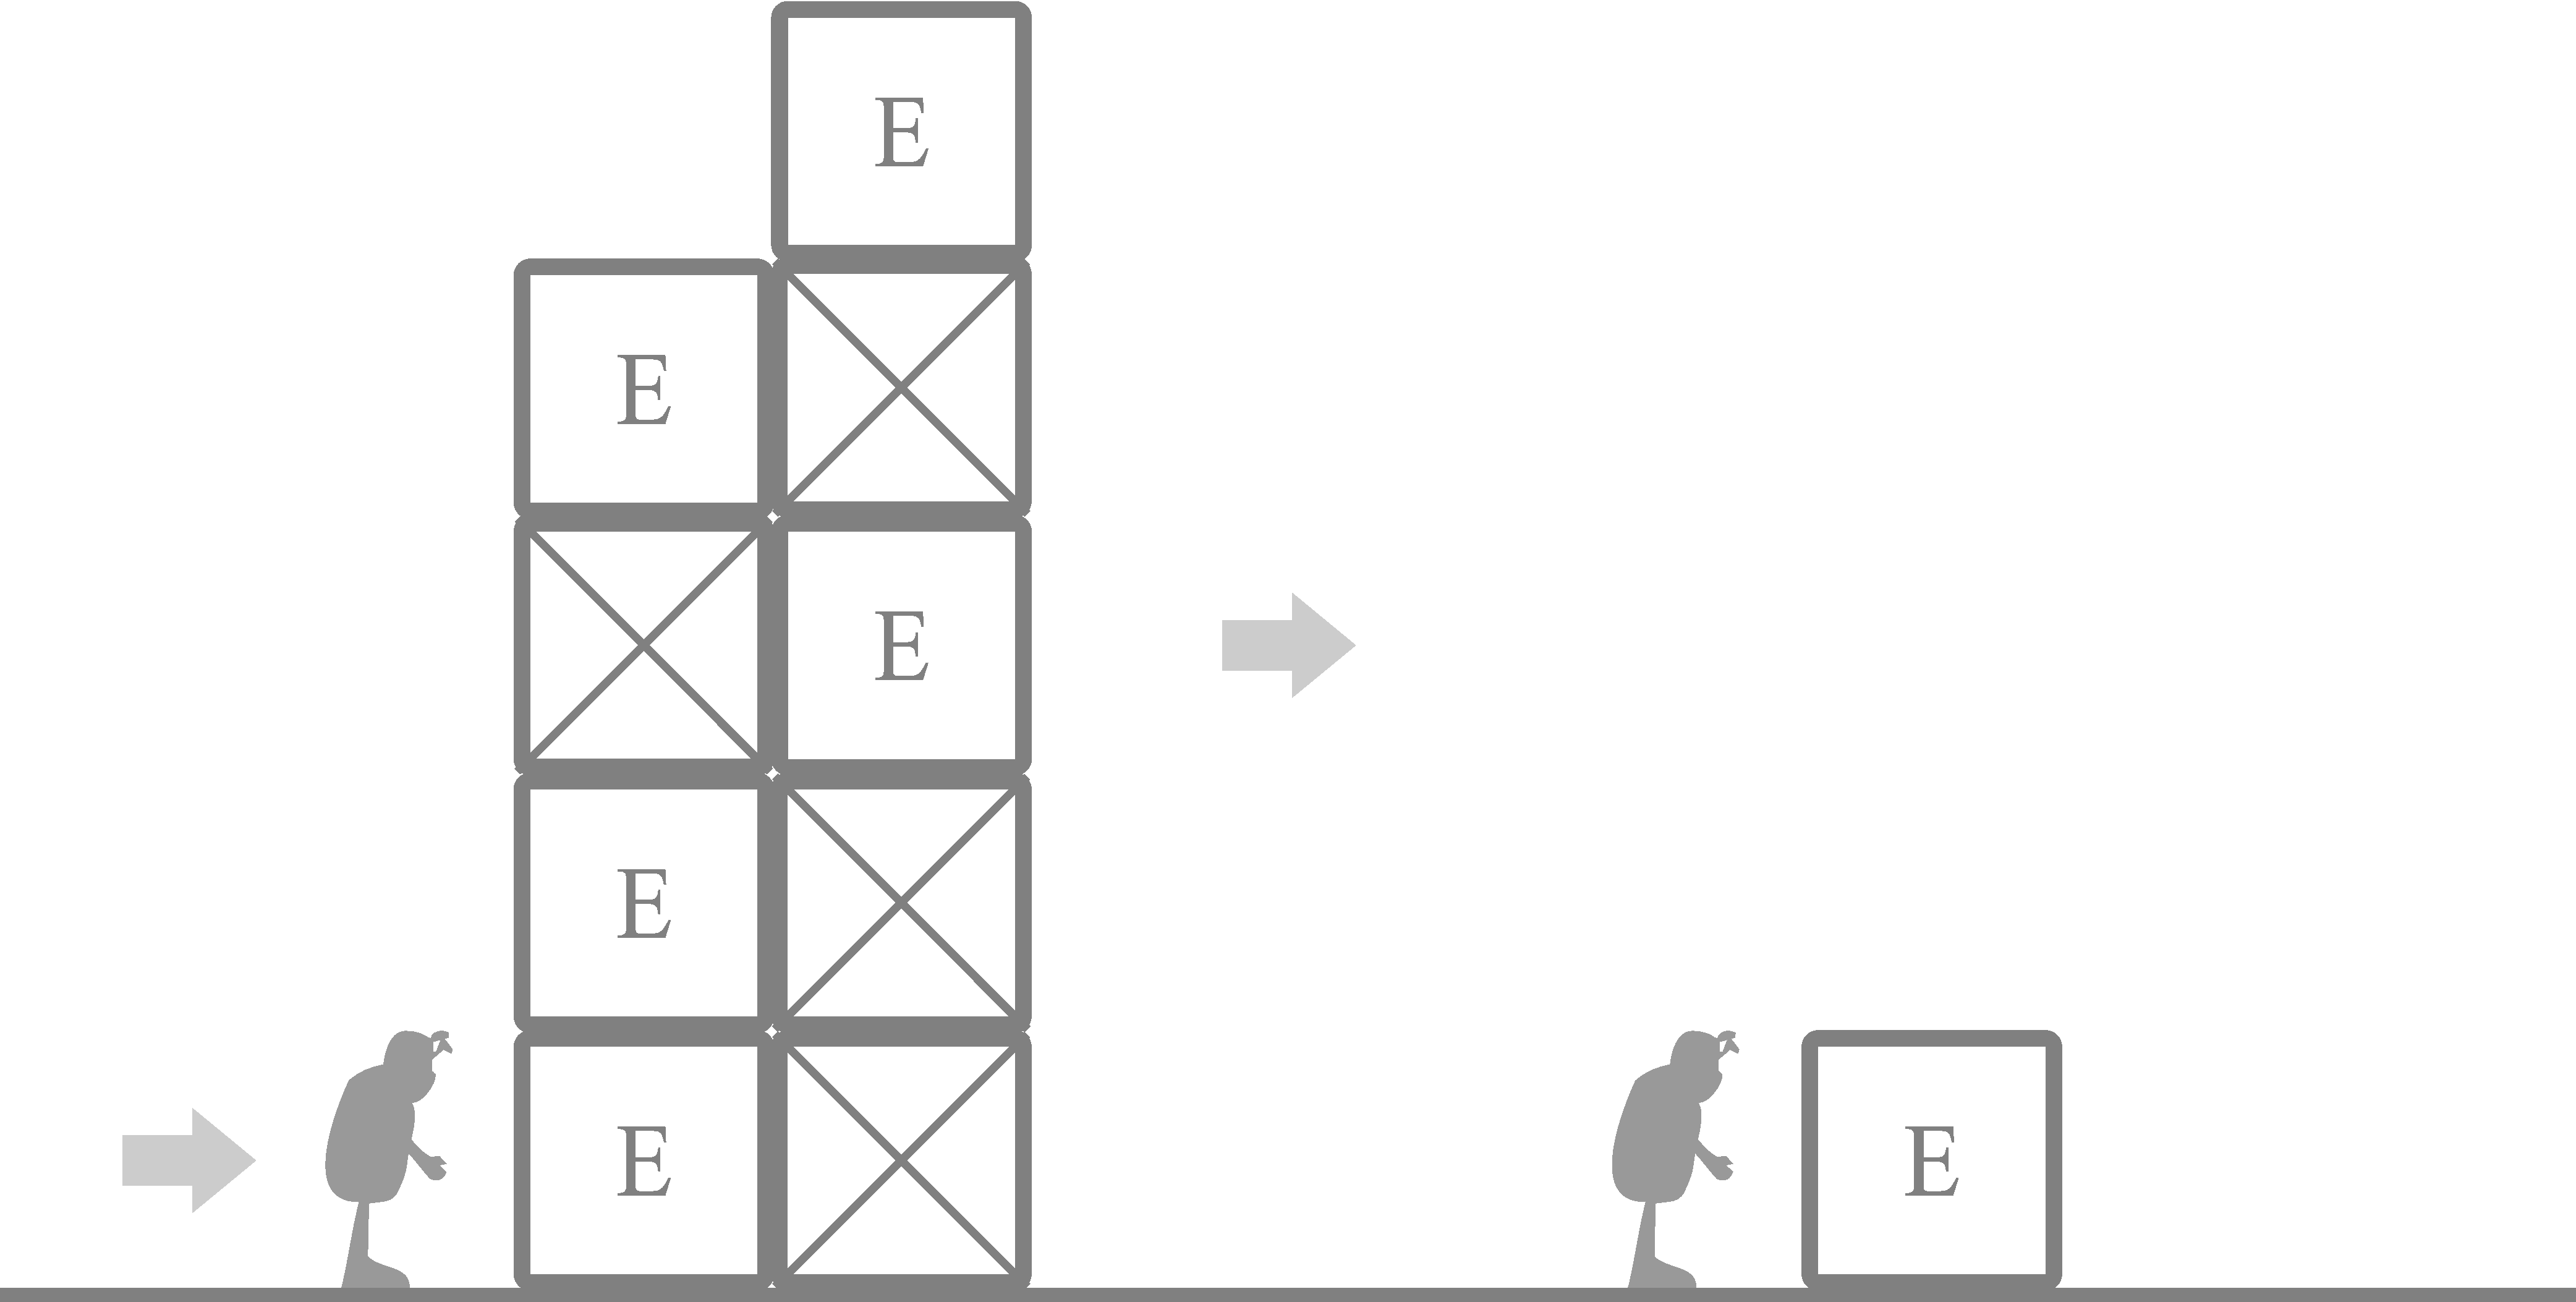
\includegraphics[width=0.8\textwidth]{bangDiagram}
\caption{Ukázka komplexního výbuchu}
\label{fig:bangDiagram}
\end{figure}

\section{Ovládání}
Berušky jsou vybírány pomocí kláves \keystroke{1} až \keystroke{5} a je s nimi pohybováno pomocí šipek. Důležité je ovládání kamery, která rotuje kolem momentálně vybrané berušky pohybem myši na okraj herní obrazovky. Pokud nemá uživatel přímou viditelnost na vybranou berušku, pak může objekty, které se mezi ním a beruškou nacházejí, nechat zprůhlednit pomocí mezerníku. Tlačítkem \Enter je pak pozice kamery přesunuta nad herní pole. 

\section{Vykreslování}
\label{section:navrhVykreslovani}
Informace týkající se technologie vykreslování jsou uvedeny v následujícím odstavci. Jejich přítomnost nechť čtenář bere pouze jako zajímavost, jelikož implementace hry, která je součástí této práce, probíhala nezávisle na hře původní. Jediným převzatým materiálem byla, jak se čtenář dále dozví, data pro zobrazení herní úrovně. 

V původní hře je celá scéna organizována jako strom hierarchických OBB obálek. Při vykreslování je pak strom procházen a je zjišťována viditelnost jednotlivých obálek. Osvětlovací model je kombinovaný z per-vertex shadingu a lightmap. Hra obsahuje také mnohé animace, které jsou u berušek realizovány jako objektové a pro zbytek objektů scény jako mesh animace. Aktuálně vyvíjená open-source varianta hry obsahuje také například zrcadlový rendering, kreslení odlesků, halo efekty, anisotropické filtrování textur, bump-mapping, komprimované textury a mip-mapping. Informace o uvedených technologiích vykreslování zde nebudou z důvodu omezeného rozsahu této práce uvedeny.

\section{Návrh webu}
Implementace této části nebyla přímou součástí této práce, a proto jejímu návrhu nebude věnován velký prostor. Návrh webu je možné vidět na diagramu~\ref{fig:web}. Web je rozdělen na 3~části a jejich popis se nachází v následujících odstavcích.


\subsection*{Menu}
Pomocí menu se volí kontexty obrazovky (viz. dále).
\subsection*{Obrazovka} Obrazovka je primárně určena k zobrazení aktuálně načtené herní úrovně. Pro ucelenost webu je však obrazovka využita i k zobrazení dalších informací a lze tedy rozpoznávat její jednotlivé kontexty. Těmi jsou:
	\begin{itemize}
	\item Hra

\item Informace o hře
\item Návod na hraní hry
\item Popis ovládání hry
	\end{itemize}
Při volbě herního kontextu se v rámci obrazovky zobrazí samotný element \texttt{<canvas>}, do kterého je vykreslována zvolená herní úroveň. V levém dolním rohu je zobrazen inventář aktuálně vybrané berušky a v rohu pravém je možné ovládat přehrávání herní hudby. Reakce na události vytvářené hráčem jsou zpracovány a o některých z nich je zobrazena notifikace, která tak dává hráči zpětnou vazbu. 
\subsection*{Výběr herních úrovní}
Tato část umožňuje uživateli vybrat z dostupných herních úrovní, které jsou následně vykreslovány do herního kontextu obrazovky. Mezi jednotlivými bloky pro výběr úrovně lze přecházet poklikem na šipky. Při jednom pokliku jsou úrovně posunuty o jeden blok a při pokliku dvojitém pak o bloky 4. Výběr by neměl obtěžovat hráče v okamžiku, kdy není potřeba. Proto je možné ho otevřít/skrýt pomocí tlačítka, které je umístěno ve spodní části obrazovky.



\chapter{Implementace}
\label{chap:implementace}
V kapitole~\ref{chap:analysis} byla analyzována hra Berušky 2, která se stala vzorem pro hru implementovanou v rámci této práce. Způsob, jakým je hra implementována, je uveden na diagramu~\ref{fig:gameDiagram}. V následující podkapitolách budou popsány jeho jednotlivé části a tím i objasněna herní architektura.

TODO...jak byla testovana funkcnost

\begin{figure}[htb]
\centering
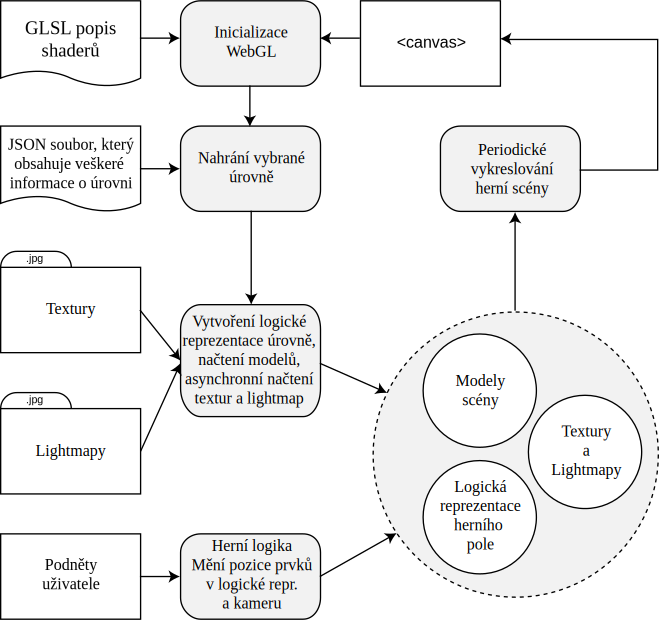
\includegraphics[width=0.8\textwidth]{gameDiagram}
\caption{Architektura hry Berušky 2 WebGL}
\label{fig:gameDiagram}
\end{figure}

\section{Inicializace}
Inicializace elementu \texttt{<canvas>} je prvním krokem, který je potřeba vykonat. Tím, že získáme referenci na jeho \texttt{webgl} kontext, můžeme přejít k dalšímu kroku, který nastaví vertex a fragment shadery. Popis funkčnosti shaderů je proveden pomocí jazyka GLSL, jehož ukázky byly uvedeny u popisu grafické pipeline (\ref{subsection:pipeline}). Zdrojové kódy jsou obsaženy v HTML dokumentu uvnitř těchto elemtentů:
\begin{itemize}
\item Vertex Shader \\ \texttt{\textless script id="per-fragment-lighting-vs"\ type="x-shader/x-vertex"\textgreater}
\item Fragment Shader \\ \texttt{\textless script id="per-fragment-lighting-fs"\ type="x-shader/x-fragment"\textgreater}
\end{itemize}

V implementaci je hra inicializována pomocí funkce \texttt{webGLStart()}, která mimo jiné nastavuje způsob zpracování událostí vytvářených uživatelem.

\section{Nahrání vybrané úrovně}
Po inicializaci je přistoupeno k nahrání úrovně vybrané hráčem. Každá z úrovní je představována samostatným JSON souborem, který je asynchronně nahrán (\ref{subsection:AJAX}) ze serveru.

\subsection*{JSON soubor}
\label{subsection:navrhJSON}
Tento soubor obsahuje kompletní informace, které jsou potřebné pro zobrazení dané herní úrovně. Jedná se tak o hlavní součást celé hry, bez které by nemohla fungovat. Soubor vzniká exportem potřebných informací z původní hry a jeho hlavní součásti jsou popsány v následujících odstavcích.

\myparagraph{Informace o materiálech}
Materiály jsou použity k otexturování modelů. Rozdíl mezi materiálem a texturou je takový, že materiál se obecně může skládat z více textur, které se pak vzájemně prolínají. Lze tak mít například materiál, který vznikne složením z textur zdi a mechu. Výhoda je v tom, že složitější textury lze složit z jednodušších a není tedy potřeba uchovávat nadbytečná data. Každý z materiálů má v souboru jména textur, ze kterých se skládá, a také své unikátní jméno, pomocí něhož se následně objekty scény na tento materiál odkazují. Ukázka popisu materiálu je uvedena ve zdrojovém kódu~\ref{code:jsonMaterial}.

\begin{lstlisting}[caption=Objekt \texttt{material} vstupního souboru JSON,label=code:jsonMaterial]
{
  "type" : "material",
  "name" : "256_p-d1-256",
  "transparent" : "0",
  "z_buffer_mask" : "1",
  "z_buffer_test" : "1",
  "backface_culling" : "1",
  "diffuse_color" : "1",
  "specular_color" : "0",
  "textures" : [ "s1_0013.jpg" ]
}
\end{lstlisting}

\myparagraph{Obálky objektů herní scény}
Málokterý ze složitějších objektů je složen pouze z jednoho modelu. Ve chvíli, kdy celkový model objektu rozdělíme na části, je možné tyto části samostatně transformovat či měnit materiál, který používají. Avšak v okamžik, kdy chceme nějakým způsobem transformovat celý objekt, je vhodné mít všechny modely objektu v jakési obálce. Tato obálka má v souboru své identifikační číslo, které slouží k identifikaci všech jejích modelů. Identifikační číslo je potřebné pouze tehdy, pokud potřebujeme s obálkou transformace provádět a je tedy využito pouze u dynamických objektů herní plochy.

\mysubparagraph{Modely}
Modely jsou v souboru reprezentovány strukturami, které obsahují informace o poloze modelů v rámci scény, o jejich barvě či například o materiálech, které jsou jim přiřazeny. Některé z modelů mají také další textury s předpočítanými stíny pro realističtější zobrazení scény - lightmapy. 

Ve zdrojovém kódu~\ref{code:jsonContainer} je uveden zjednodušený popis obálky, která obsahuje 1 model. Identifikační číslo \texttt{2} znamená, že se jedná o dynamický prvek scény (pokud by se jednalo o statický prvek, pak by číslo bylo \texttt{-1}). Pomocí položky \texttt{material} se model v tomto případě odkazuje na materiál, který byl popsán ve zdrojovém kódu~\ref{code:jsonMaterial}. Trojice prvků v poli \texttt{vertexPositions} vždy udává pozici vertexu ve scéně. O tom, které vertexy náleží geometrickým primitivám, ze kterých je model složen, rozhoduje pole \texttt{indices}. Zbylé položky pak obsahují informace potřebné pro správné namapování materiálů a lightmap.

\begin{lstlisting}[caption=Objekt \texttt{geometry\_container} vstupního souboru JSON,label=code:jsonContainer]
{
  "type" : "geometry_container",
  "name" : "exit.b2m",
  "container_id" : "2",
  "poly_id" : "17",
  "prvek" : "1",
  "geometry_objects" : [
   {
    "name" : "exit.b2m",
    "material" : "256_p-d1-256",
    "vertexPositions" : [-27.586000,2.008000,-34.421001,-27.586000,0.008000,-36.421001,
         47.704437,85.772964,6.669896,130.704437,85.772964,-3.330104],
    "vertexNormals" : [-1.000000,0.000000,0.000000,-1.000000,0.000000,0.000000],
    "vertexTextureCoords0" : [1.000000,1.000000,0.000000,0.000000,1.000000,0.000000],
    "vertexTextureCoords1" : [1.000000,1.000000,0.000000,0.000000,1.000000,0.000000],
    "vertexTextureCoordsLight" : [0.140625,0.328125,0.171875,0.328125,0.156250,0.359375],
    "indices" : [0,1,2,3,0,5]
   }
  ]
}
\end{lstlisting}

\myparagraph{Logická reprezentace herního pole}
Obálky modelů neobsahují žádnou informaci o tom, jaký typ objektu ve scéně představují. Z tohoto důvodu je nutné rozlišit to, co je vykreslováno na obrazovku, a s čím pracuje logika hry. Jak již bylo uvedeno v kapitole~\ref{chap:analysis}, herní pole je krychlové či kvádrové a je složeno z jednotlivých pozic, na kterých se mohou nacházet herní prvky. Je to právě logická reprezentace herního pole, která obsahuje informace o tom, který prvek se na které pozici nachází. Každý prvek logické reprezentace herního pole má opět své identifikační číslo, pomocí kterého se odkazuje na obálku modelu, který určuje jeho vzhled.  

Ve zdrojovém kódu~\ref{code:jsonLogic} je uveden popis herního pole o velikosti $6\times6$ a výšce $8$. Položka \texttt{level\_start} udává pozici, na kterou mají být přesunuty dynamické objekty, které jsou normálně umístěny v počátku souřadného systému scény. Herní pole zde obsahuje pouze jeden prvek, jehož typ je určen položkami \texttt{class} a \texttt{subclass} (identifikátory všech prvků jsou uvedeny v tabulce~\ref{table:itemClass}). Logický prvek se v tomto příkladu pomocí \texttt{container\_id} odkazuje na model, který byl popsán ve zdrojovém kódu~\ref{code:jsonContainer}. 

\label{code:jsonLogic}
\begin{lstlisting}
{
  "type" : "level_logic",
  "logic_level_size" : [ 6, 8, 6],
  "level_start" : [ 21.586000, -1.992000, -46.421001],
  "item_size" : "2",
  "level_items_num" : "1",
  "level_items" : [{
    "name" : "Exit - teleport - 1",
    "guid" : "4000",
    "class" : "4",
    "subclass" : "-1",
    "position" : [ 0, 5, 1 ],
    "rotation" : "0",
    "container_id" : "2"
  }]
}
\end{lstlisting}

\begin{table}
\label{table:itemClass}
\begin{center}
\begin{tabular}{ | l | l | l |}
\hline
\textbf{Prvek} & \textbf{itemClass} & \textbf{itemSubclass} \\ \hline
Beruška & 1 & 0 \\ \hline
Zeď & 2 & 0 \\ \hline
Východ & 4 & 0 \\ \hline
Bedna & 5 & 0 \\ \hline
Těžká bedna & 5 & 0 \\ \hline
Lehká bedna & 5 & 1 \\ \hline
Výbušnina & 6 & 0 \\ \hline
Kámen & 7 & 0 \\ \hline
Voda & 12 & 0 \\ \hline
Šnorchl & 13 & 0 \\ \hline
Hormonální vitamín & 13 & 5 \\ \hline
Závaží & 13 & 7 \\ \hline
Krompáč & 13 & 8 \\ \hline
Bortící se podlaha & 15 & 0 \\ \hline
Šikmina & 19 & 0 \\ \hline
\end{tabular}
\end{center}
\caption{Třídy a podtřídy prvků herního pole}
\end{table}

Jak si mohl pozorny čtenář všimnout, čísla, která označují typ prvku, nejdou sekvenčně za sebou. Je to způsobeno tím, že původní návrh hry Berušky 2 (desktopové verze) obsahoval více typů herních prvků, než jich bylo nakonec implementováno. 

\section{Vytvoření vnitřní reprezentace herní úrovně}
Každé struktuře vyskytující se v JSON souboru (popsáno v~\ref{subsection:navrhJSON}) přísluší odpovídající objekty a po jeho asynchronním načtení je soubor zpracován pomocí funkce \texttt{handleLoadedJSON}. Ta tento soubor sekvenčně prochází, rozpoznává jeho jednotlivé struktury a následně pomocí JavaScriptových konstruktorů vytváří odpovídající objekty, se kterými hra pracuje. V následujících odstavcích je uveden přehled těchto konstruktorů s jejich stručným popisem.

\myparagraph{\texttt{Material}}
Při vytváření objektu tímto konstruktorem jsou ze serveru asynchronně (\ref{subsection:AJAX}) nahrány textury, které materiál využívá. Z těch jsou následně vytvořeny texturovací buffery, které jsou nahrány do grafické paměti. Tím, že jsou do této paměti umístěny, je pak dosaženo rychlejšího vykreslování celé herní scény. Buffery jsou nastaveny tak, že pokud je textura oproti své původní velikosti zvětšována (upscaling), pak se použije lineární filtr, který na základě okolních pixelů dopočítá lineární interpolací barvu pixelu mezi nimi. Pro textury, které jsou naopak zmenšovány je vygenerována mipmapa, ze které se pak vybírá nejvhodnější verze textury. Všechny materiály jsou uchovávány v asociativním poli \texttt{materials}, kde jednotlivé klíče tohoto pole jsou samotné názvy materiálů. 

Ve zdrojovém kódu~\ref{code:loadingMaterial} je uveden příklad nahrání texturovacího bufferu vzniklého načtením první textury materiálu uvedeného ve zdrojovém kódu~\ref{code:jsonMaterial} do grafické paměti.

\begin{lstlisting}[caption=Příklad nahrání textury do grafické paměti,label=code:loadingMaterial]
// ...	
// Textura je zrcadlově obrácena kolem osy Y
// WebGL používá jiný souřadný systém
gl.pixelStorei(gl.UNPACK_FLIP_Y_WEBGL, true);
// Nastavení aktuálně zpracovávaného bufferu textury
gl.bindTexture(gl.TEXTURE_2D, materials["256_p-d1-256"].buffers[0]); 
// Nahrání textury do grafické paměti
gl.texImage2D(gl.TEXTURE_2D, 0, gl.RGBA, gl.RGBA, gl.UNSIGNED_BYTE, 
              that.textures[temp].image);
// Nastavení filtru, kterým bude textura zvětšována
gl.texParameteri(gl.TEXTURE_2D, gl.TEXTURE_MAG_FILTER, gl.LINEAR);
// Nastavení filtru, kterým bude textura zmenšována
gl.texParameteri(gl.TEXTURE_2D, gl.TEXTURE_MIN_FILTER, 
                 gl.LINEAR_MIPMAP_NEAREST);
// Vygenerování mipmapy
gl.generateMipmap(gl.TEXTURE_2D);
// ...
\end{lstlisting}

\myparagraph{\texttt{Lightmap}}
Objekt vytvořený tímto konstruktorem je až na pár detailů stejný jako objekt konstruktoru \texttt{Material}. Lightmapy jsou taktéž načítány asynchronně a ukládány do paměti grafické karty, avšak vzhledem k tomu, že se z původní hry nepodařilo všechny lightmapy vyexportovat, je jejich použití vypnuto.

\myparagraph{\texttt{GeometryContainer}}
\label{paragraph:obálky}
Tento konstruktor vytváří obálku jednotlivých modelů herní scény. Podle toho, zda obálka obsahuje identifikační číslo, rozlišujeme mezi obálkami dynamických a statických objektů scény a umísťujeme je do odpovídajících polí. Pro dynamické obálky je to asociativní pole \texttt{dynamicItems}, jehož klíči jsou identifikátory obálek a pro statické obálky je to pole staticItems, kde jsou obálky seřazeny tak, jak byli načítány ze vstupního souboru. Každá z obálek ve svém poli \texttt{objects} uchovává modely, které jí náleží. 

\myparagraph{\texttt{GeometryObject}} 
Objekt vytvořený tímto konstruktorem obsahuje veškeré informace spojené s vykreslováním modelu. Důležité je to, že jsou zde uloženy buffery, do kterých jsou nahrány informace o pozicích vertexů, směrech jejich normál a dále pak například o souřadnicích potřebných pro správné namapování materiálu. Ve zdrojovém kódu~\ref{code:vertexBuffer} je uveden příklad nahrání pozic vertexů ze struktury, která v JSON souboru reprezentuje načítaný model.

\begin{lstlisting}[caption=Příklad nahrání pozic vertexů do bufferu,label=code:vertexBuffer]
// Vytvoření vertex position bufferu
this.vertexPositionBuffer = gl.createBuffer();
gl.bindBuffer(gl.ARRAY_BUFFER, this.vertexPositionBuffer);
// Načtení dat z JSON souboru
gl.bufferData(gl.ARRAY_BUFFER, new Float32Array(model.vertexPositions), 
              gl.STATIC_DRAW);
this.vertexPositionBuffer.itemSize = 3;
this.vertexPositionBuffer.numItems = model.vertexPositions.length / 3;
\end{lstlisting}

\myparagraph{\texttt{Logic}}
\label{paragraph:logic}
Objekt tohoto konstruktoru obsahuje veškeré informace spojené s herním polem a také veškerou herní logiku. Prvky herního pole jsou reprezentovány objekty konstruktoru \texttt{LogicItem}. Vzhledem ke svému rozsahu je tento objekt popsán samostatně v podkapitole~\ref{section:implementationLogic}.

\myparagraph{\texttt{LogicItem}}
Objekty představují jednotlivé herní prvky, které obsahují informace o jejich typu, pozici a aktuálním natočení. Každý z prvků má své unikátní identifikační číslo, které slouží k propojení s obálkou jeho modelu.

\section{Herní logika a podněty uživatele}
\label{section:navrhLogika}
V implementované hře je každý podnět uživatele zpracováván herní logikou, která je implementována na základě analýzy hry Berušky 2 provedené v kapitole~\ref{chap:analysis}. Pro vyhodnocení podnětu uživatele je volána funkce \texttt{gameStep()}. Ta představuje herní krok, ve kterém je vždy zjištěna pozice aktuálně zvolené berušky a dle jejího natočení se pak určí pozice, na kterou hodlá přejít. Podle toho, jaký typ prvku se na následující pozici nachází, jsou vykonávány akce, jejichž popis je uveden v následujícím přehledu.

\begin{itemize}
\item \textbf{Nic} - pokud je beruška v nejnižší úrovní herního pole, pak je krok proveden. Pokud ne, pak je nejdříve zkontrolován obsah pozice, která je pod místem, kam hodlá beruška přejít.
\begin{itemize}
\item Pod místem je \textit{šikmina}. Pokud je šikmina správně natočena, pak se ještě zkontroluje, zda nevede šikmina pod vodní hladinu, kde by beruška potřebovala šnorchl. Při splnění všech podmínek je krok následně proveden.
\item Pod místem je \textit{bortící se podlaha}. Ta se propadne pouze v případě, že má beruška ve svém inventáři závaží.
\item Pod beruškou je jiná \textit{beruška} - přechod se neprovede.
\item Pokud zde není \textit{žádná pevná plocha}, na které by beruška mohla stát (zeď, bedna, východ, výbušnina či kámen), pak se krok neprovede. 
\end{itemize}
\item \textbf{Beruška} - krok se neprovede, jinou beruškou nelze přímo pohnout.
\item \textbf{Zeď} - krok se neprovede, zeď je statickým prvkem herního pole.
\item \textbf{Východ} - beruška opouští herní pole. Pokud je to beruška poslední, pak končí hra.
\item \textbf{Bedna} - zjistí se celková váha všech posouvaných beden a pokud je nižší nebo rovna beruščině síle, pak se bedna/bedny v daném směru posouvají. Pokud pod sebou posunutá bedna nemá podklad, pak je její pozice upravena tak, aby ho pod sebou měla.
\item \textbf{Výbušnina} - zjistí se, co se nachází na pozici, kam by měla být výbušnina posunuta. Pokud je na následující pozici bedna, pak je výbušnina i bedna odstraněna a beruška zůstává na své původní pozici. Pokud za výbušninou není bedna, pak se stejně jako bedna posune.
\item \textbf{Kámen} - prohledá se inventář berušky a pokud obsahuje krompáč, pak je kámen odstraněn s tím, že beruška zůstává na své původní pozici. V opačném případě se krok neprovede.
\item \textbf{Šnorchl} - beruška může vlastnit pouze jeden. Pokud ho tedy ještě ve svém inventáři nemá, pak se šnorchl odstraní z herního pole, přidá se do beruščina inventáře a ta samotná je posunuta na pozici, kde se šnorchl nacházel.
\item \textbf{Hormonální vitamín} - situace je obdobná jako u šnorchlu.
\item \textbf{Závaží} - opět stejná situace jako u šnorchlu.
\item \textbf{Krompáč} - krompáč se odstraní a přidá se do inventáře pouze v případě, že v něm má beruška místo. Maximální počet krompáčů, který může mít beruška v jeden okamžik v inventáři je 4.
\item \textbf{Bortící se podlaha} - může se nacházet i před beruškou, avšak krok který by vedl k tomu, že by beruška byla pod podlahou se neprovede.
\item \textbf{Šikmina} - zde opět záleží na natočení šikminy. Vzhledem k tomu, že se nad šikminou může nacházet jakýkoliv jiný herní prvek, je krok při správném natočení šikminy rozdělen na 2 fáze. Nejprve je beruška pro potřeby výpočtu přesunuta nad šikminu a následně je krok prováděn z tohoto umístění. 
\end{itemize}

Je také důležité připomenout, že při každém posunu prvků je potřeba zkontrolovat, zda se posunem nedostaly do místa, kde by levitovaly ve vzduchu. Pozice se musí upravit s tím, že pokud se v nově vzniklém sloupci prvků nachází některé výbušné bedny, pak při úpravě vertikální polohy sloupce výbušné bedny odstraňují normální bedny, které mají pod sebou. Stejně tak je potřeba kontrolovat, zda se v nově vzniklém sloupci prvků nenachází bortící se podlaha. Pokud je váha nad bortící se podlahou vyšší jak 1, pak je bortící se podlaha odstraněna a sloupec objektů je vertikálně posunut.

\subsection*{Objekt herní logiky}
\label{section:implementationLogic}
Při vytvoření tohoto objektu jsou z JSON souboru načteny potřebné informace a podle nich jsou pak dopočítány ty zbylé. Prvky herního pole se stejně jako obálky modelů (\ref{paragraph:obálky}) dělí na statické a dynamické a jsou uloženy v odpovídající polích \texttt{staticItems} a \texttt{dynamicItems} tohoto objektu (neplést s poli určenými pro obálky modelů, které jsou uloženy v globálních polích se stejnými názvy). Statické prvky jsou indexovány pomocí čísla, které je odvozeno z pořadí při jejich načítání. Dynamické prvky jsou naopak indexovány svým identifikačním číslem. 

Jak již bylo uvedeno v~\ref{paragraph:logic}, tento objekt obsahuje veškerou herní logiku v podobě funkcí, které jsou rozděleny do několika kategorií. Kategorie a odpovídající komentované přehledy jsou uvedeny v tabulce~\ref{table:logicCategories}.

\begin{table}
\label{table:logicCategories}
\begin{center}
\begin{tabular}{ | l | l |}
\hline
\textbf{Kategorie} & \textbf{Zdrojový kód} \\ \hline
Práce s beruškami & \ref{code:logicBug} \\ \hline
Práce s inventářem & \ref{code:logicInventory}\\ \hline
Získávání reference na prvky & \ref{code:logicReference}\\ \hline
Výpočet váhy prvků & \ref{code:logicWeight} \\ \hline
Posun prvků & \ref{code:logicMove} \\ \hline
Odstraňování prvků & \ref{code:logicRemove} \\ \hline
Herní krok & \ref{code:logicGameStep}\\ \hline
\end{tabular}
\end{center}
\caption{Kategorie funkcí herní logiky}
\end{table}

\begin{lstlisting}[caption=Funkce pro práci s beruškami,label=code:logicBug]
/**
* Vybere berušku s daným ID.
* @param id ID berušky, která má být vybrána
*/
function selectBug(id) {/*...*/}
/** 
* Vybere následující berušku.
*/
function selectNextBug() {/*...*/}
/**
* Odstraní berušku z hracího pole.
* Po odstranění poslední berušky končí hra.
* @param id ID berušky, která má být odstraněna
*/
function removeBug(id){/*...*/}
/**
* Posune berušku na zadanou pozici a navíc
* zjistí, zda se pod beruškou nenacházelo propadlo.
* Pokud ano, pak se zjistí aktuální váha nad propadlem
* a propadlo se případně odstraní.
* @param id Identifikační číslo berušky
* @param position Pozice, na kterou má být beruška přesunuta
*/
function moveBug(id, position){/*...*/}
\end{lstlisting}

\pagebreak

\begin{lstlisting}[caption=Funkce pro práci s beruščiným inventářem,label=code:logicInventory]
/**
* Ověří, zda se v inventáři berušky nachází daný předmět.
* @param bugID Identifikační číslo berušky
* @param itemSubclass Podtřída vyhledávaného předmětu
* @return -1 pokud nebyl předmět nalezen, nebo pozici předmětu v inventáři
*/
function inventoryContains(bugID, itemSubclass){/*...*/}
/**
* Přidá předmět do beruščina inventáře.
* @param bugID Identifikační číslo berušky
* @param itemSubclass Podtřída přidávaného předmětu
*/
function inventoryAppend(bugID, itemSubclass){/*...*/}
/**
* Odebere předmět z berušcina inventáře.
* @param bugID Identifikační číslo berušky
* @param itemPosition Pozice odebíraného předmětu v inventáři
*/
function removeFromInventory(bugID, itemPosition){/*...*/}
\end{lstlisting}

\begin{lstlisting}[caption=Funkce pro získávání reference na prvky herního pole,label=code:logicReference]
/** 
* Získá referenci na prvek hracího pole, který se nachází na dané pozici.
* @param position Pozice prvku
*/
function getObjectOnPosition(position) {/*...*/}
/** 
* Získá referenci na prvek hracího pole s daným ID.
* @param id Identifikátor prvku.
*/   
function getObjectByID(id) {/*...*/}
/** 
* Získá pozici prvku se zadaným id.
* @param id Identifikátor prvku
*/
function getPositionOfObject(id) {/*...*/}  
\end{lstlisting}

\begin{lstlisting}[caption=Funkce pro výpočet váhy objektů,label=code:logicWeight]
/**
* Získá váhu prvku na zadané pozici.
* Jakmile se jedná o statický prvek, pak jeho váha 1000.
* @param position Pozice objektu
*/
function getWeightOfObject(position) {/*...*/}    
/** 
* Vypočítá váhu sloupce od zadané pozice nahoru.
* @param position Pozice, od které má výpočet probíhat
*/
function getWeightOfColumn(position){/*...*/}  
/** 
* Sečte váhu herních prvků v daném směru. Pracuje rekurzivně.
* @param direction Směr - up, right, down, left
* @param position Pozice od, které má být výpočet proveden
*				  obvykle pozice, na následující pozice berušky
*/
function countWeight(direction, position){/*...*/} 
\end{lstlisting}

\begin{lstlisting}[caption=Funkce pro posun objektů,label=code:logicMove]
/**
* Posune prvek herního pole a s ním i všechny
* prvky, které se nachází nad ním.
* Jakmile je posun ukončen, jsou upraveny vekrtikální pozice
* prvků tak, aby pod sebou měli podklad.   
function moveObject(direction, tempObject){/*...*/}
/**
* Rekurzivně posouvá prvky herníno pole.
* K posuvu využívá funkci moveObject a je volána
* teprve tehdy, když už je jisté, že prvky lze
* posunout - nejdříve se počítá váha posouvaného bloku
* @param direction Směr posunu - up, right, down, left
* @param position Pozice, od které má být posuv proveden
*                 Obvykle následující pozice berušky
*/ 
function moveAction(direction, position){/*...*/}
\end{lstlisting}

\begin{lstlisting}[caption=Funkce pro odstraňování objektů,label=code:logicRemove]
/**
* Odstranní prvek herního pole.
* Nejprve je odstraněn model prvku a poté jeho záznam v logické reprezentaci.
* @param item Reference na prvek, který má být odstraněn
*/
function removeItem{/*...*/}
\end{lstlisting}

\begin{lstlisting}[caption=Funkce herního kroku gameStep,label=code:logicGameStep]
/**
* Veškerý pohyb ve hře je zprostředkován pomocí této funkce.
* Vypočítá následující pozici berušky, určí typ předmětu na této
* pozici a podle typu se rozhoduje, jaké kroky provést.
*
* Tato funkce přijímá jeden z parametrů.
* Buď je jím směr, kterým se aktuálně vybraná beruška má vydat,
* nebo je to přímo pozice, na kterou hodlá beruška přejít.
* Přímé pozice je využito například u šikminy, kde beruška nemění
* svou pozici pouze o 1 krok, avšak je nutné berušku posunout nad/pod
* šikminu. 
* @param direction Směr, kterým se vybraná beruška vydává.
* @param newBugPositionIn Pozice, na kterou se beruška chystá jít.
*/
function gameStep(direction, newBugPositionIn) {/*...*/}
\end{lstlisting}
\pagebreak
\section{Ovladání}
Hra je ovládána pomocí klávesnice a myši. Při stisku jakékoliv klávesy je zjištěn její kód, kterým je identifikována v rámci JavaScriptu a dle tohoto kódu je prováděna příslušná akce.

Existují dva způsoby, kterými lze reagovat na stisknuté klávesy: 
\begin{itemize}
\item Reagovat ihned na událost stisku klávesy,
\item Pravidelně kontrolovat aktuálně stisknuté klávesy a provádět příslušné operace.
\end{itemize}   

Pro uživatele je rozdíl takový, že pokud drží klávesu, tak v prvním případě již po první reakci nenásledují žádné další. V případě druhém se pak akce opakovaně provádějí do té doby, dokud uživatel klávesu drží, avšak za tu cenu, že nemusí být zachyceny všechny stisky kláves. Ze spolehlivostních důvodů je tedy v implementaci zvolen první způsob reakce. 

Klávesy a odpovídající akce na jejich stisk jsou uvedeny v tabulce~\ref{table:keys}.

\begin{table}
\label{table:keys}
\begin{center}
\begin{tabular}{ | l | l |}
\hline
\textbf{Klávesa} & \textbf{Akce klávesy}\\ %\hline
\UArrow & Pohyb aktuálně vybrané berušky - provádění herního kroku \\ %\hline
\LArrow & Natočení berušky o 90\degree vlevo \\ %\hline
\RArrow & Natočení berušky o 90\degree vpravo \\ %\hline
\DArrow & Otočení berušky o 180\degree \\ %\hline
\keystroke{1} & Výběr berušky 1 \\
\keystroke{2} & Výběr berušky 2 \\
\keystroke{3} & Výběr berušky 3 \\
\keystroke{4} & Výběr berušky 4 \\
\keystroke{5} & Výběr berušky 5 \\
\keystroke{m} & Změna vykreslovacího módu \\ %\hline
\keystroke{n} & Přepíná mezi vykreslováním celé scény a samotného herního pole \\ %\hline
\keystroke{c} & Změna typu kamery  \\ %\hline
\keystroke{x} & Zapíná/vypíná zobrazení lightmap \\ %\hline
\keystroke{l} & Zapíná/vypíná použití bodového světla \\ %\hline
\keystroke{f} & Přepíná mezi zobrazením přes celou obrazovku a normálním zobrazením \\ %\hline
\keystroke{o} & Zapíná/vypíná průhlednost objektů \\ %\hline
\keystroke{s} & Zapíná/vypíná zobrazení odlesků \\ %\hline
\keystroke{r} & Restartuje herní úroveň \\ %\hline
\Enter & Přepíná mezi horním pohledem a pohledem normálním \\ \hline

\end{tabular}
\end{center}
\caption{Ovládání hry pomocí klávesnice}
\end{table}

Myší je ovládána kamera. Tlačítko \keystroke{c} slouží k přepínání různých typů kamery, kterými jsou: 

Kamera má více možností zobrazení:

\begin{itemize}
\item Kamera s bodem otáčení kolem středu herního pole
\item Kamera s bodem otáčení kolem aktuálně vybrané berušky
\item Pohled berušky
\item Pohled na záda berušky
\end{itemize}

U prvních dvou typů zobrazení je kamera ovládána pomocí myši tak, jak možné vidět na diagramu~\ref{fig:web}. Herní obrazovka je rozdělena na oblasti, které jsou citlivé na kurzor myši. Najetím kurzoru myši je následně změněn úhel rotace kamery a její elevace. U zbylých dvou typů kamery je rotace a elevace pevně určena aktuální pozicí a rotací berušky. WebGL nemá přímou podporu pro kameru. Výsledný pohled nevzniká tedy tak, že by se transformovala pozice a natočení kamery v rámci scény, avšak je vytvořen tak, že kamera je umístěna na pevné pozici a pohybuje se celou scénou. To, jakým způsoben je toto implementováno, je uvedeno v podkapitole~\ref{implementace:vykreslovani}. 

\section{Vykreslování}
\label{implementace:vykreslovani}
Vykreslování probíhá periodicky s tím, že modely scény jsou při vykreslování transformovány na základě aktuálních informací, které se nacházejí v logické reprezentaci herní úrovně. Původní hra obsahuje animace prvků herního pole a svého okolí. V implementované hře animace nejsou obsaženy a všechny transformace objektů scény jsou tedy prováděny ihned po dokončení herního kroku. Jedná se o zjednodušení, které bylo odsouhlaseno již při zadávání projektu.  

Vykreslování obstarává funkce \texttt{drawScene()}. Na počátku této funkce je vždy vyčištěn color a depth buffer a následně je přistoupeno k vytvoření projekční matice a matice kamery

Projekční matice je nastavena na úhel projekce 45\degree. Je však možné ho po nastavení proměnné \texttt{useProjection} měnit tlačítky \keystroke{[} a \keystroke{]}. Reset projekční matice se pak provádí pomocí tlačítka \keystroke{'}. Další nastavení hry je uvedeno v podkapitole~\ref{section:nastaveni}.

Matice kamery je sestavena na základě jejího aktuálně zvoleného typu. Vytvoření této matice se skládá z několika kroků:

\begin{itemize}
\item Vytvoření $4\times4$ matice identity \texttt{cameraMatrix}
\item Translace této matice v osách X a Z - určí se střed otáčení kamery
\item Rotace kolem osy Y - aplikuje rotaci vlevo, nebo vpravo
\item Rotace kolem osy X -  aplikuje aktuální elevaci
\item Translace kolem osy Z - posune kameru od středu otáčení.
\end{itemize}

Jelikož není maticové násobení komutativní operací, je nutné provádět transformace v tomto pořadí. Po sestavení matice kamery je vzhledem k tomu, že pohybujeme scénou a ne kamerou, vytvořena matice k ní inverzní. Tou je vynásobena tzv. \textit{model-view} matice, kterou jsou následně násobeny všechny vertexy, které se ve scéně nacházejí. Vykreslování se řídí následujícím algoritmem.


\pagebreak
\begin{algorithmic}
\label{algorithm:vykreslovani}
\ForAll{(obálka in pole\_obálek)} \\ 
Ulož model-view matici
\If{((frustrum culling) AND (obálka není viditelná ve frustru kamery))} \\ \quad \quad continue \EndIf
\If{((obálka není součástí herního pole) \&\& (není zobrazena celá scéna))} \\ \quad \quad continue \EndIf
	\ForAll{(model in obálka)}
		\If{((frustrum culling) AND (model je ve frustru kamery))} \\ \quad \quad \quad \quad continue \EndIf
		\If{((model má průhledný materiál) OR (je zapnut blending))} \\ \quad \quad \quad \quad přidej objekt do pole \texttt{blendedObjects}, continue\EndIf
		\If{(zapnuto použití textur)} \\ \quad \quad \quad \quad Nahraj texturu používanou modelem do pipeline \EndIf
		\If{((zapnuto použití lightmap) AND (model má lightmapu))} \\ \quad \quad \quad \quad Nahraj lightmapu používanou modelem do pipeline  \EndIf	\\
    	\If{(dynamický prvek scény)} \\ \quad \quad \quad \quad Proveď trasnsformace model-view matice dle logické reprezentace \EndIf	\\
	    \quad \quad \quad Nahraj buffer s vertexy do pipeline \\
		\quad \quad \quad Nahraj buffer s normálami vertexů do pipeline \\ 
		\quad \quad \quad Nahraj model-view matici do pipeline \\ 
		\quad \quad \quad Vykresli modely za použití aktuálně zvoleného typu vykreslování \\
	\EndFor \\
Nahraj uloženou model-view matici
\EndFor
\end{algorithmic} 
\medskip

Algoritmem jsou procházeny jednotlivé obálky statických či dynamických objektů a je testováno, zda náleží do oblasti viditelné pozorovateli. Pokud není ani jeden bod obálky v této oblasti, pak nejsou její modely vykreslovány. Se zapnutým vykreslováním celé scény je další test přeskočen, avšak v případě, že tomu tak není, je testováno, zda je obálka prvkem herního pole. V dalším cyklu se již procházejí jednotlivé modely obálky, které jsou opět testovány na svou viditelnost. Jakmile jsou viditelné, pak je potřeba získat informaci o tom, zda není jejich materiál částečně průhledný, nebo zda nebyli zprůhledněny všechny vykreslované objekty. Pokud se tedy jedná o model s průhledným materiálem, pak je jeho vykreslování odloženo na pozdější dobu. Jakmile jsou splněny další podmínky, pak jsou nahrány textury/lightmapy a je přistoupeno k samotnému vykreslování. Model-view matice, která vznikla složením z invertované matice kamery a transformací, které byly provedeny na základě informací v logické reprezentaci scény, je nahrána do grafické pipeline a s ní i vertexy modelu a jejich normály. Modely jsou následně vykresleny tak, jak bylo popsáno v podkapitole~\ref{section:webgl}. 

V implementované hře jsou obálky modelů rozděleny na statické a dynamické, takže vykreslování probíhá ve více samostatných cyklech. Navíc je ještě při zobrazení samotného herního pole vykreslována podlaha. Při zobrazení modelů s průhledným materiálem dojde k odloženému vykreslování modelů v samostatném cyklu. Jednotlivé vykreslovací cykly jdou tedy v tomto pořadí:


\myparagraph{1. Vykreslení podlahy herního pole}
Podlaha herního pole je vykreslována v případě, že je zobrazeno pouze samotné hrací pole (klávesa \keystroke{n}). Umístění vertexů a pozice textury podlahy jsou vypočítány vždy při vytvoření objektu s logickou reprezentací úrovně.
\myparagraph{2. Vykreslení statických objektů}
Statické objekty jsou uchovány v poli \texttt{staticItems} a není u nich potřeba provádět transformaci model-view matice, jelikož se vůči scéně nacházejí stále na stejné pozici.
\myparagraph{3. Vykreslení dynamických objektů}
Dynamické objekty jsou umístěny v asociativním poli \texttt{dynamicItems} a jsou umisťovány na pozice, které odpovídající jejich pozici v logické reprezentaci scény. Výsledná translace v jednotlivých osách je vypočítána podle následujícího vztahu.
\begin{align}
translace_{xzy}  = start_{xyz} + pozice_{xyz} * velikostPozice
\end{align}
Proměnná $start_{xyz}$ je místo, na kterém se nachází pozice $[0,0,0]$ herního pole. Proměnná $pozice_{xyz}$ udává pozici herního pole, kde se nacházi aktuálně vykreslovaný model a $velikostPozice$ je konstantou, která udává, jak velká je jedna pozice herního pole v souřadném systému scény. 

\myparagraph{4. Vykreslení průhledných objektů}
Některé z herních úrovní obsahují modely, které mají průhledné materiály. Tyto modely musí být vykresleny až po modelech, které průhledné nejsou. Vykreslování průhledných objektů se dále komplikuje tím, že k tomu, abychom byli schopni zkombinovat barvy materiálů a dosáhli tak efektu průhlednosti, musíme modely nejdříve seřadit podle jejich vzdálenosti od pozorovatele. Jako první jsou vykresleny modely nejvzdálenější a nakonec ty, které jsou k pozorovateli nejblíže. Při načítání jednotlivých modelů z JSON souboru jsou také dopočítávány jejich středy, které jsou právě při tomto řazení využity. Je důležité si uvědomit, že seřazení modelů musí proběhnout při každém volání vykreslovací funkce, a tudíž je následný propad v rychlosti vykreslování poměrně znatelný. Barvy materiálů jsou pak kombinovány v části grafické pipeline, která byla popsána v podkapitole~\ref{section:webgl}. Průhlednost všech objektů scény lze zapnout pomocí klávesy \keystroke{o}.

\pagebreak
\myparagraph{Osvětlení}
Výsledný obraz je také určen osvětlením z různých světelných zdrojů, které se ve scéně nacházejí. Stejně tak jako chybí podpora pro práci s kamerou, chybí ve WebGL i podpora osvětlení. Veškeré výpočty jsou tedy prováděny \uv{ručně}, a to přímo v shaderech grafické karty. V implementaci je využito phongova osvětlovacího modelu, který oproti osvětlovacímu modelu původní hry používá per-fragment shading\footnote{Intenzita osvětlení fragmentu nevzniká interpolací intenzit osvětlení vertexů, ale je počítána pro každý fragment zvlášť. Je tak dosaženo více realistického typu zobrazení scény.}. Využito je pouze jednoho dynamického bodového světla, které je umístěno přímo nad herním polem. Implementace jako taková je připravena na využití více světel, avšak při navýšení jejich počtu exponenciálně klesá výkonnost vykreslovaní. Osvětlení lze zapnout pomocí klávesy \keystroke{l} a odlesky pomocí klávesy \keystroke{s}. Vzhledem k omezenému rozsahu práce se již nebudeme osvětlením dále zabývat. 

\section{Nastavení hry}
\label{section:nastaveni}
Některé způsoby nastavení již byli uvedeny v předchozím textu. V tabulce~\ref{table:settings} je uveden přehled nejdůležitějších proměnných, které mění způsob, jakým se chová vykreslování herní scény. Kompletní přehled je obsažen ve vygenerované dokumentaci, která je součástí přiloženého DVD.

\begin{table}
\label{table:settings}
\begin{center}
\begin{tabular}{ | l | l |}
\hline
\textbf{Proměnná} & \textbf{Použití} \\ \hline
\texttt{drawOnlyGameField} & Zapnutí vykreslení celé scény \\ \hline
\texttt{useOpacity} & Zprůhlednění všech objektů scény \\ \hline
\texttt{opacityLevel} & Nastavení úrovně průhlednosti objektů scény \\ \hline
\texttt{useTextures} & Zobrazení textur \\ \hline
\texttt{useLightmaps} & Zobrazení lightmap \\ \hline
\texttt{useLightning} & Zapnutí osvětlení \\ \hline
\texttt{useSpecular} & Zobrazení odlesků \\ \hline
\texttt{useTopCamera} & Přepne na kameru kolmou herní pole \\ \hline
\texttt{paintSelectedBugRed} & Beruška zčervená po jejím vybrání  \\ \hline
\texttt{drawEnvelopes} & Vykreslení obálek dynamických objektů scény  \\ \hline
\texttt{drawFloor} & Vykreslení podlahy \\ \hline
\texttt{useNotifications} & Zobrazení notifikací \\ \hline
\texttt{showFPSinConsole} & Zobrazí FPS v konzoli prohlížeče \\ \hline
\texttt{useProjection} & Zapnutí možnosti změny úhlu projekce\\ \hline
\texttt{log} & Zobrazení debugovacích informací v konzoli prohlížeče \\ \hline
\texttt{renderMode} & Nastavení typu vykreslování \\ \hline
\texttt{cameraMode} & Nastavení typu kamery \\ \hline
\end{tabular}
\end{center}
\caption{Některá z herních nastavení}
\end{table}
\chapter{Testování}
\label{chap:testing}
Tato kapitola se primárně zabývá testováním implementované hry. Jeho výsledky jsou důležité pro následnou diskuzi ohledně využitelnosti nově objevujících webových technologií. K tomu, abychom mohli takovou diskuzi provádět, je nejprve potřeba porovnat výsledné řešení s původní hrou a představit tak výhody/nevýhody webu nativních aplikací.

\section*{Porovnání her}
Implementovaná hra zakládá na hře Berušky 2. Herní koncept zůstal zachován, avšak způsob, jakým je řešeno vykreslování, je odlišný. Původní hra je technologicky mnohem vyspělejší (viz.~\ref{section:navrhVykreslovani}). Obsahuje animace, řeší viditelnost objektů scény pomocí hierarchických OBB obálek a využívá mnoho dalších moderních technologií. Hra je oproti implementované i výrazně rychlejší. Při rozlišení $1920x1080$ dosahuje hra rychlosti 52 snímků za sekundu a při rozlišení $1024x768$ 124 snímků za sekundu~\footnote{Intel x3100}. Implementované řešení má tedy v oblasti vykreslování mnoho prostoru ke zdokonalení a optimalizaci. Implementovaná hra však vítězí v dostupnosti. Je možné ji bez instalace začít ihned používat na většině dnešních operačních systémů. Byla ověřena funkčnost i na operačním systému Android. Hru na tomto systému však není možné ovládat, jelikož nepřijímá dotykové události. Výslednou podobu hry Berušky 2 WebGL v prohlížeči Firefox 12 je možné vidět na obrázku~\ref{fig:gameImage}. 

\section*{Testování}
Hra byla testována v prohlížečích Mozilla Firefox a Google Chrome na operačním systému Microsoft Windows 7. Testy byly provedeny na dvou různých strojích s rozdílnou hardwarovou konfigurací.

\begin{itemize}
\item Intel C2D T7100, GPU Intel x3100
\item Intel C2D T5700, GPU ATI Radeon 4330
\end{itemize}

Rozdílnost těchto strojů tkví hlavně v instalované grafické kartě. Intel x3100 neumí používat shader model 2.0, který je nutností pro hardwarovou akceleraci WebGL. Obraz je tedy vykreslován softwarově. Hra byla vždy testována se zapnutým zobrazením celé scény a následně se zobrazením samostatného herního pole. Každý z testů je navíc proveden pro různé velikosti drawing bufferu~\ref{subsection:pipeline} a různé vykreslovací módy. Hodnoty v polích tabulek vždy udávají vykreslené snímky za sekundu\footnote{FPS}.

\myparagraph{Intel x3100}

\begin{table}[!ht]
\begin{center}
\begin{tabular}{ | r | c | c | c | c |}
\hline
 & \multicolumn{2}{|c|}{$896 \times 504$} & \multicolumn{2}{|c|}{$1920 \times 979$} \\ \hline
 & \textbf{Herní pole} & \textbf{Celá scéna} & \textbf{Herní pole} & \textbf{Celá scéna} \\ \hline
\textbf{Plné zobrazení} & 15 & 3 & 7 & 2 \\ \hline
\textbf{Žádné odlesky} & 15 & 3 & 7 & 2 \\ \hline
\textbf{Bez textur} & 16 & 3 & 7 & 2 \\ \hline
\textbf{Bez osvětlení} & 16 & 3 & 7 & 2 \\ \hline
\textbf{Bez textur a osvětlení} & 17 & 3 & 7 & 3 \\ \hline
\end{tabular}
\end{center}
\caption{Windows 7, Intel x3100, Firefox 11.0}
\end{table}

\begin{table}[!ht]
\begin{center}
\begin{tabular}{ | r | c | c | c | c |}
\hline
 & \multicolumn{2}{|c|}{$896 \times 504$} & \multicolumn{2}{|c|}{$1920 \times 979$} \\ \hline
 & \textbf{Herní pole} & \textbf{Celá scéna} & \textbf{Herní pole} & \textbf{Celá scéna} \\ \hline
\textbf{Plné zobrazení} & 51 & 17  & 35 & 13 \\ \hline
\textbf{Žádné odlesky} & 51 & 17  & 35 & 13 \\ \hline
\textbf{Bez textur} & 51 & 17& 35 & 13 \\ \hline
\textbf{Bez osvětlení} & 51 & 17 & 48 & 17 \\ \hline
\textbf{Bez textur a osvětlení} & 56 & 18 & 50 & 17 \\ \hline
\end{tabular}
\end{center}
\caption{Windows 7, Intel x3100, Chrome 19.0.1084.46}
\end{table}

\myparagraph{ATI Radeon 4330}

\begin{table}[!ht]
\begin{center}
\begin{tabular}{ | r | c | c | c | c |}
\hline
 & \multicolumn{2}{|c|}{$896 \times 504$} & \multicolumn{2}{|c|}{$1920 \times 979$} \\ \hline
 & \textbf{Herní pole} & \textbf{Celá scéna} & \textbf{Herní pole} & \textbf{Celá scéna} \\ \hline
\textbf{Plné zobrazení} & 60 & 37 & 44 & 32 \\ \hline
\textbf{Žádné odlesky} & 60 & 37 & 44 & 32 \\ \hline
\textbf{Bez textur} & 60 & 39 & 51 & 38 \\ \hline
\textbf{Bez osvětlení} & 60 & 40 & 44 & 32 \\ \hline
\textbf{Bez textur a osvětlení} & 60 & 41 & 43 & 40 \\ \hline
\end{tabular}
\end{center}
\caption{Windows 7, Chrome 19.0.1084.46, ATI Radeon 4330}
\end{table}

\begin{table}[!ht]
\begin{center}
\begin{tabular}{ | r | c | c | c | c |}
\hline
 & \multicolumn{2}{|c|}{$896 \times 504$} & \multicolumn{2}{|c|}{$1920 \times 979$} \\ \hline
 & \textbf{Herní pole} & \textbf{Celá scéna} & \textbf{Herní pole} & \textbf{Celá scéna} \\ \hline
\textbf{Plné zobrazení} & 46 & 4 & 31 & 4 \\ \hline
\textbf{Žádné odlesky} & 46 & 4 & 31 & 4 \\ \hline
\textbf{Bez textur} & 47 & 4 & 33 & 4 \\ \hline
\textbf{Bez osvětlení} & 49 & 4 & 32 & 4 \\ \hline
\textbf{Bez textur a osvětlení} & 50 & 41 & 34 & 4 \\ \hline
\end{tabular}
\end{center}
\caption{Windows 7, Firefox 11, ATI Radeon 4330}
\end{table}

Rozdíl softwarového a hardwarového vykreslování obrazu není příliš znatelný. Není ani vidět příliš velký rozdíl v rychlosti vykreslování různých typů zobrazení. Rozdíl je však znatelný v rychlosti prohlížečů Firefox 11 a Chrome 19. Google Chrome je obecně známý tím, že obsahuje velice rychlý interpret JavaScriptového kódu. Bylo také provedeno testování v prohlížeči Google Chrome 9, což je první verze tohoto prohlížeče, která podporovala technologii WebGL. Obraz nebyl vykreslován rychlostí vyšší než 2 snímky za sekundu a lze tedy u tohoto prohlížeče vidět výrazný posun k lepšímu.

Z poznatků, které byly při testech získány je možné vidět velikou závislost rychlosti vykreslování na rychlosti zpracování JavaScriptového kódu. I když se rychlost interpretace JavaScriptového kódu neustále zvyšuje, není tento jazyk stále určen pro zpracování velkého množství dat. Pro optimalizaci WebGL aplikací je tedy potřeba přenechat co největší část práce na grafickém hardwaru. 

Na prvním uvedeném systému byla také testována byla také rychlost načítání herní úrovně. Původní hra načetla úroveň za 9 sekund. Herní úroveň hry implementované v této práci se v prohlížeči Chrome 19 načítá 30 milisekund. Z toho se 20 milisekund načítá JSON soubor a 10 milisekund se načítají potřebné textury. V této situaci však byly veškeré herní soubory uloženy lokálně. Doba potřebná k zobrazení úrovně ze serveru je výrazně vyšší. JSON soubor obsahuje mnoho informací a jeho průměrná velikost se pohybuje kolem 6 MB. Jsou však i takové herní úrovně, které s texturami zabírají kolem 15 MB dat. Čtenář si jistě dokáže představit, jak dlouhou dobu načítání takového množství dat trvá.
\chapter{Závěr}
\label{chap:zaver}
V rámci této bakalářské práce byla analyzována hra Berušky 2, na jejímž základě byl následně vytvořen návrh a implementace webové hry Berušky 2 WebGL. K vývoji bylo využito moderních webových technologií, které byly stručně představeny a uvedeny do souvislosti s jejich použitím. Veškerá funkčnost implementovaného řešení byla popsána pomocí jazyků JavaScript a GLSL pro popis shaderů grafické karty. Implementované řešení bylo podrobeno testům, jejichž výsledky byly diskutovány s konzultantem této práce - Ing. Martinem Stránským. Je důležité zdůraznit, že řešení rozšiřuje zadání práce o různé možnosti nastavení vykreslování, implementaci webu, přehrávání herní hudby a mnohá vylepšení v podobě animací, které vylepšují celkový dojem z celé aplikace.

Po konzultaci s panem Ing. Martinem Stránským byly použité technologie celkově zhodnoceny jako vhodné pro vývoj aplikací jako je ta, jejíž implementace byla součástí této práce. Pro komerční využití je však potřeba, aby byli nejprve odstraněny některé problémy, které jsou spojené s tím, že web a jeho prostředky nebyly pro tyto účely vytvořeny. WebGL například používá hardwarové akcelerace vykreslování, avšak aplikace využívající toto rozhraní stále nedosahují rychlosti aplikací desktopových. To, co podle provedených testů WebGL \textit{brzdí}, je výpočetní rychlost JavaScriptu. JavaScript není určen pro operace s velkým množstvím dat. Interprety tohoto jazyka jsou však dnes středem pozornosti a lze tedy předpokládat, že tento problém bude postupně mizet.

Existuje velké množství technik sloužících k zobrazení realisticky vypadající herní scény. Tato hra některé z nich implementuje, avšak stále zbývá mnoho prostoru pro optimalizace a vylepšení. Jednou z optimalizací, se kterou se hra v brzké době setká, je tzv. frustrum culling, pro nějž je hra již částečně připravena. Další je redukce přenášených dat. Pokud by to technologie umožnily, pak by bylo pro hráče jistě přívětivé, kdyby si mohl hru spustit z lokálního úložiště a nebyl tak závislý na datovém připojení. Pokud by se technologie vyhovující tomuto účelu objevila, pak bude její využití jednou z priorit. Při konzultacích s panem Stránským byla také navržena mnohá vylepšení v tom, jakým způsobem je hra ovládána. Tato vylepšení s ním budou dále diskutována.
 % viz. obsah.tex

  % Pouzita literatura
  % ----------------------------------------------
\ifczech
  \bibliographystyle{czechiso}
\else 
  \bibliographystyle{plain}
%  \bibliographystyle{alpha}
\fi
  \begin{flushleft}
  \bibliography{literatura} % viz. literatura.bib
  \end{flushleft}
  \appendix
  
  %\chapter{Obsah CD}
%\chapter{Manual}
%\chapter{Konfigra�n� soubor}
%\chapter{RelaxNG Sch�ma konfigura�n�ho soboru}
%\chapter{Plakat}

\chapter{Diagram HTML 5 API}
\label{priloha:html5}
\begin{figure}[htb]
\centering
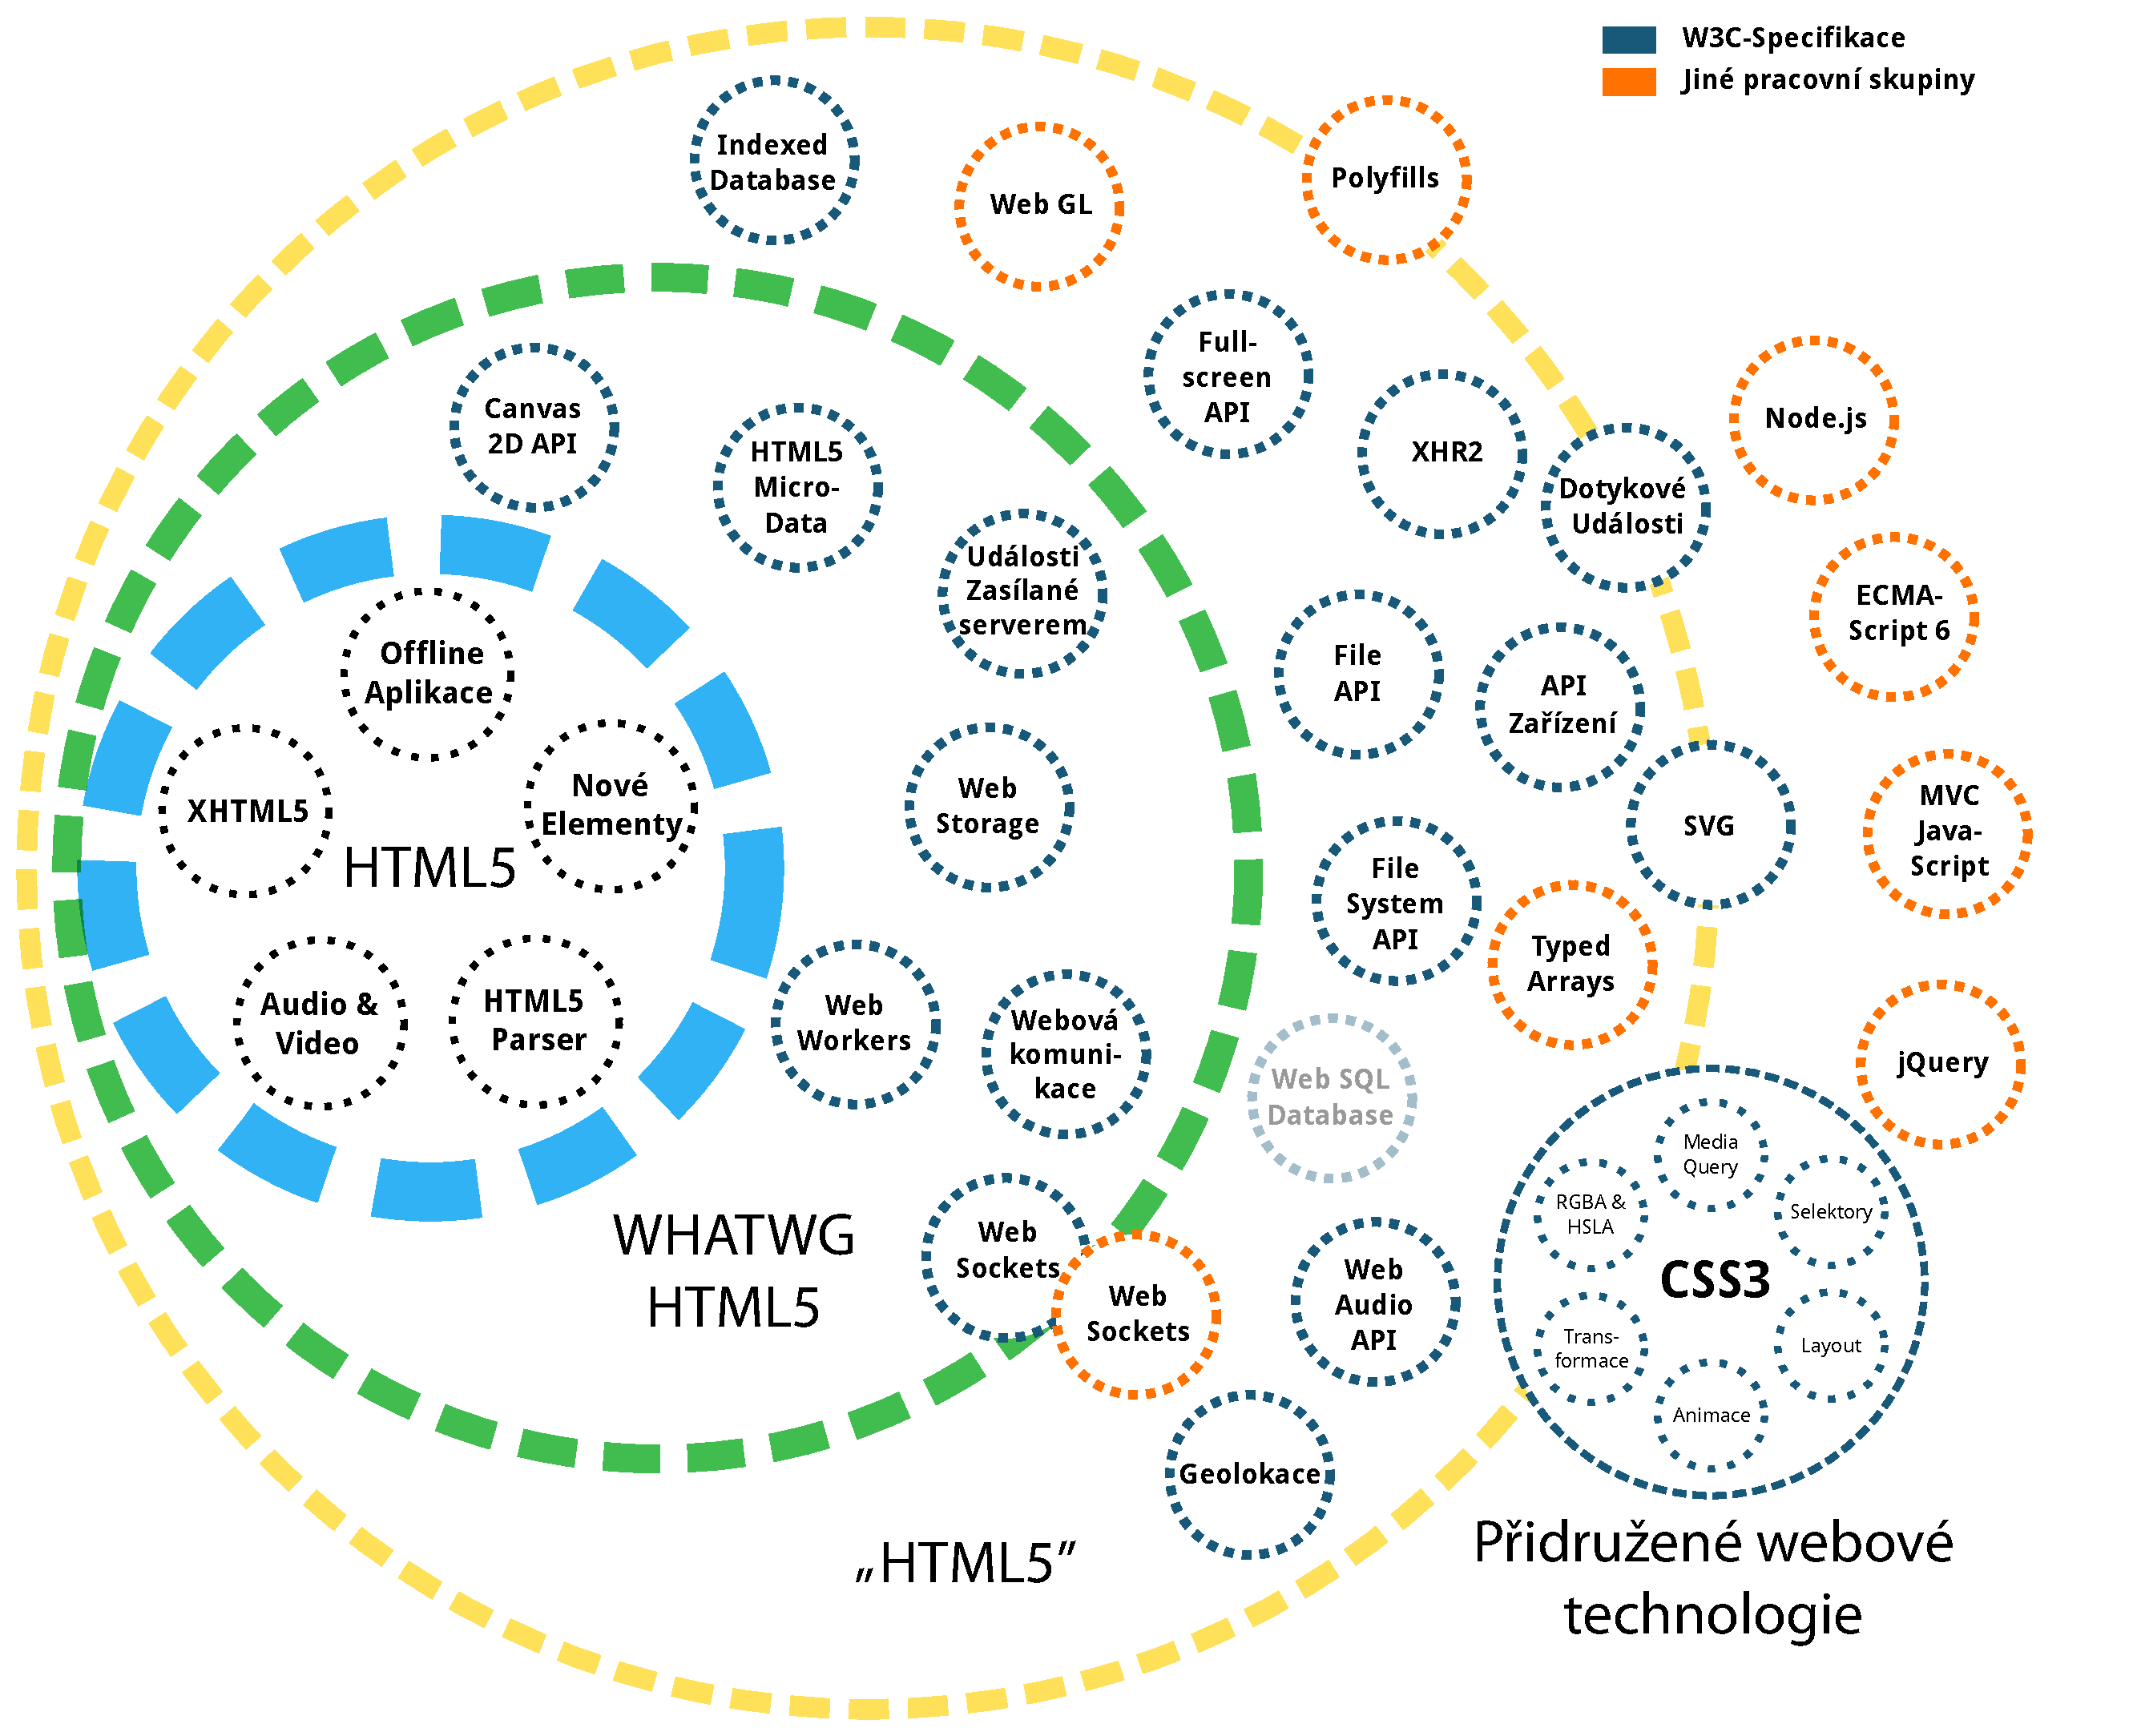
\includegraphics[width=1.0\textwidth]{html5api}
\caption{HTML 5 API}
\label{fig:html5api}
\end{figure}

\chapter{Diagram n�vrhu webu}
\begin{figure}[htb]
\centering
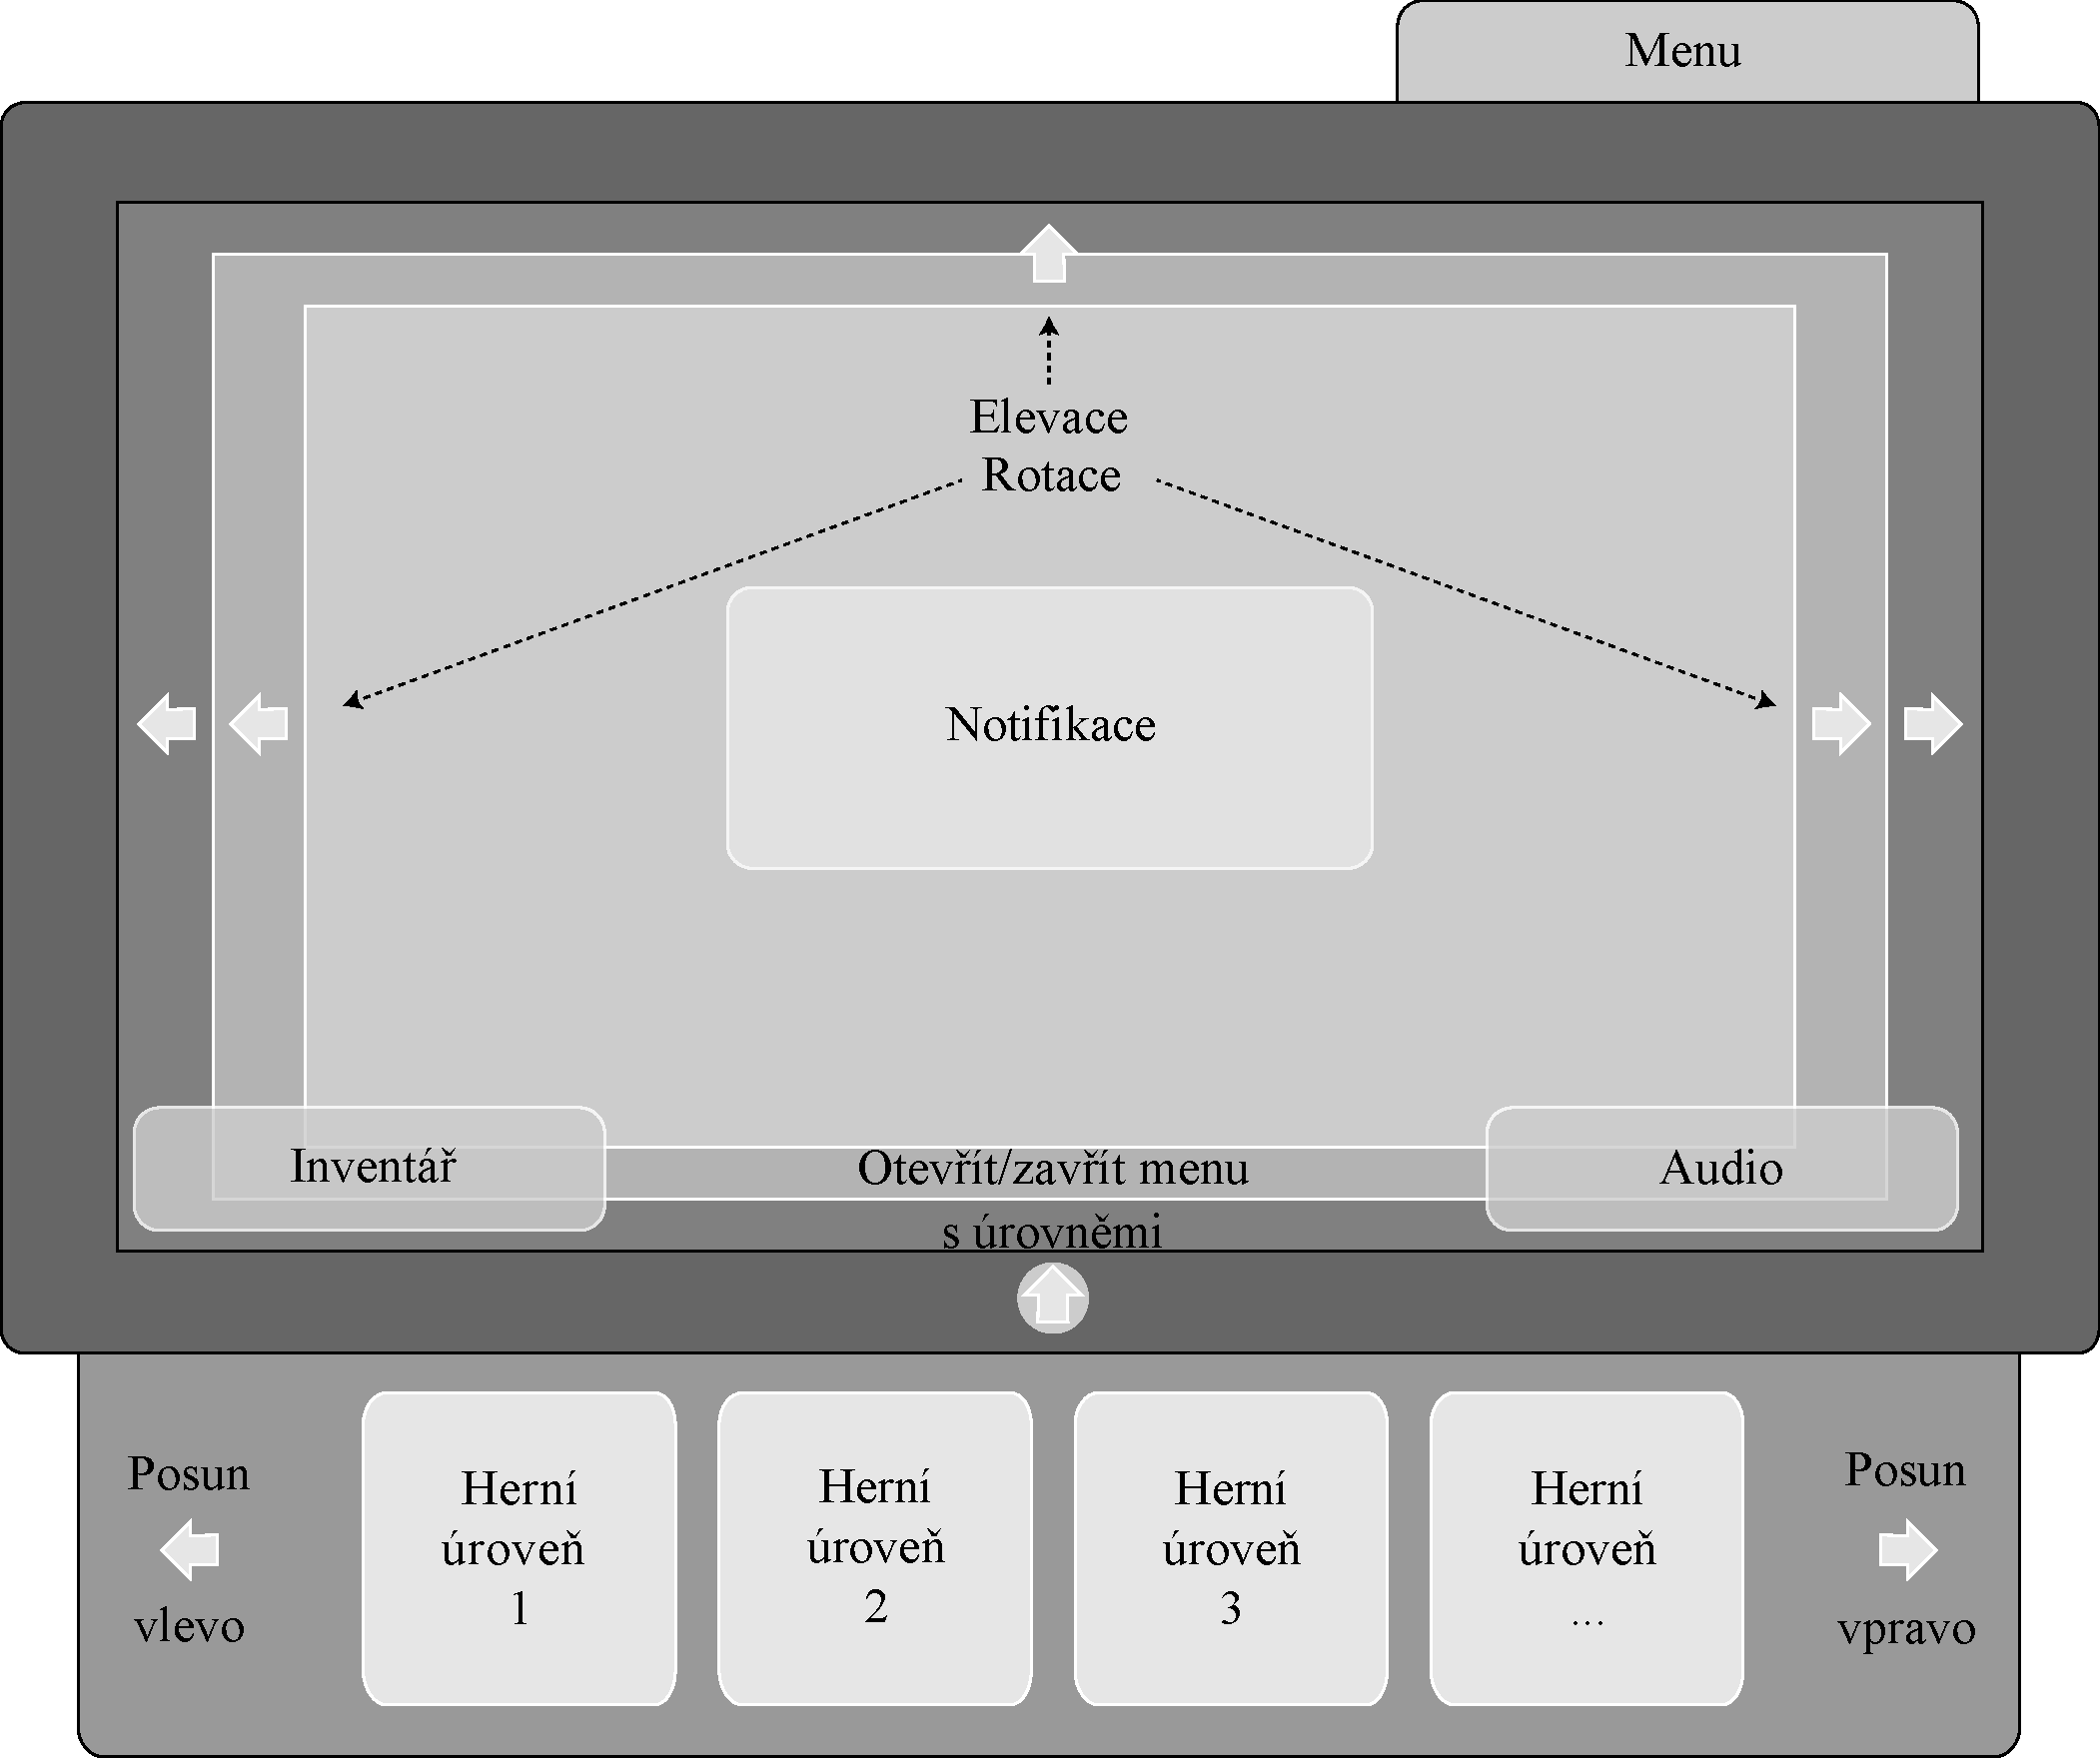
\includegraphics[width=1.0\textwidth]{web}
\caption{N�vrh webu}
\label{fig:web}
\end{figure}

%\chapter{Diagram ovl�d�n� kamery}
%\begin{figure}[htb]
%\centering
%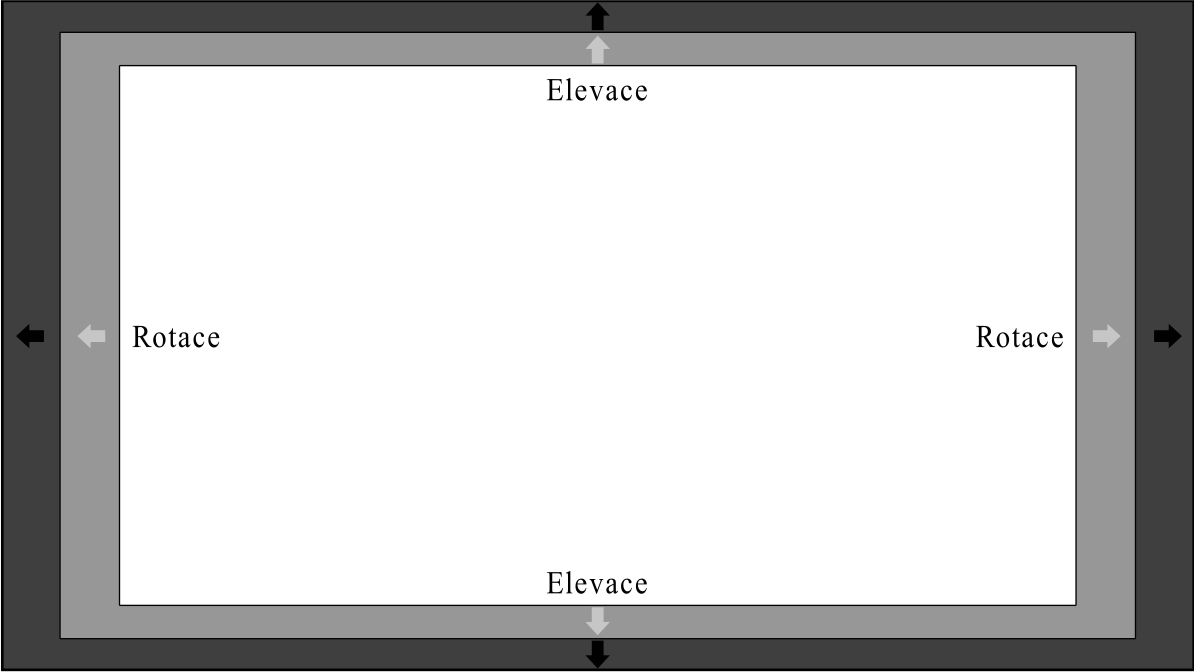
\includegraphics[width=1.0\textwidth]{mouseCamera}
%\caption{Ovl�d�n� kamery}
%\label{fig:mouseCamera}
%\end{figure}

\chapter{Podoba hry Beru�ky 2 WebGL}
\begin{figure}[htb]
\centering
\includegraphics[width=1.0\textwidth]{bugEscapeWebGL}
\caption{Beru�ky 2 WebGL v prohl��e�i Firefox 12}
\label{fig:gameImage}
\end{figure}

\chapter{Obsah DVD}
\begin{table}[!ht]
\label{table:dvd}
\begin{center}
\begin{tabular}{ | l | l |}
\hline
\textbf{Cesta} & \textbf{Popis} \\ \hline
\texttt{./audio} & Hern� hudba \\ \hline
\texttt{./css} & Kask�dov� styly \\ \hline
\texttt{./doc} & Zdrojov� soubory t�to pr�ce \\ \hline
\texttt{./dochtml} & Vygenerovan� HTML dokumentace \\ \hline
\texttt{./graphics} & Zdrojov� soubory grafiky \\ \hline
\texttt{./img} & Webov� grafika \\ \hline
\texttt{./js} & Implementace hry a soubory framework� \\ \hline
\texttt{./levels} & JSON soubory hern�ch �rovn� \\ \hline
\texttt{./lightmaps} & Lightmapy \\ \hline
\texttt{./textures} & Textury \\ \hline
\textbf{\texttt{./index.html}} & HTML dokument hry s GLSL popisem shader� \\ \hline
\end{tabular}
\end{center}
\caption{Obsah DVD}
\end{table}



 % viz. prilohy.tex
\end{document}
